% !TeX spellcheck = it_IT
\documentclass[a4paper,12pt]{report}

\usepackage{alltt, fancyvrb, url}
\usepackage{graphicx}
\usepackage{algorithmic}
\usepackage[utf8]{inputenc}
\usepackage{titling}
\usepackage{fancyhdr}
\usepackage{fontenc}
\usepackage{amsmath,mathtools,algorithm}
\usepackage{amssymb}
\usepackage{longtable}
\usepackage{setspace}
\usepackage{listings}
\usepackage{color}
\usepackage{eurosym}
\usepackage{array}
\usepackage[referable]{threeparttablex}
\usepackage{pifont}
\newcommand{\cmark}{\ding{51}}
\newcommand{\xmark}{\ding{55}}

\usepackage[italian,hidelinks]{hyperref}

\usepackage[italian]{babel}
\usepackage[italian]{cleveref}

\lstdefinestyle{json}
{
	basicstyle = \footnotesize\ttfamily,
	frame = single,
	tabsize = 4
}

\lstdefinelanguage{myScala}{
	morekeywords={abstract,case,catch,class,def,%
		do,else,extends,false,final,finally,%
		for,if,implicit,import,match,mixin,%
		new,null,object,override,package,%
		private,protected,requires,return,sealed,%
		super,this,throw,trait,true,try,%
		type,val,var,while,with,yield},
	basicstyle=\ttfamily\small,
	sensitive=true,
	keywordstyle=\color{blue},
	morecomment=[l]{//},
	morecomment=[n]{/*}{*/},
	morestring=[b]",
	morestring=[b]',
	morestring=[b]"""
}


% MARGINI LARGHI
%\textwidth 6.3 in % Width of text line.
%    \textheight 9.2 in
%    \oddsidemargin 0 in      %   Left margin on odd-numbered pages.
%    \evensidemargin 0 in      %   Left margin on even-numbered pages.
%    \topmargin 0.2 in
%    \headheight 0 in       %   Width of marginal notes.
%    \headsep 0 in
%    \topskip 0 in

\pretitle{%
	\begin{center}
		\LARGE
	}
\posttitle{\end{center}}


\title{\Huge \textbf{Proxima} \\
	\vspace{10pt}
	\vspace{20pt}
}
\author{
	Gabriele Graffieti \\ \small \url{gabriele.graffieti@studio.unibo.it}
	\vspace{15pt}
	\\
	Alfredo Maffi \\ \small \url{alfredo.maffi@studio.unibo.it}
	\vspace{15pt}
	\\
	Manuel Peruzzi \\ \small \url{manuel.peruzzi@studio.unibo.it}
}

\date{}

\pagestyle{fancy}
\fancyhf{}
\fancyhead[L]{\ifthenelse{\isodd{\value{page}}}{\thepage}{\leftmark}}
\fancyhead[R]{\ifthenelse{\isodd{\value{page}}}{\leftmark}{\thepage}}
\renewcommand{\chaptermark}[1]{\markboth{#1}{}} 

\begin{document}

\maketitle
\pagenumbering{arabic}

\begin{abstract}
	\emph{Proxima} è un servizio pervasivo che mira a fornire dei servizi personalizzati agli utenti sulla base della loro identità. Esso è stato progettato ed implementato per i corsi di \emph{Pervasive Computing} e \emph{Laboratorio di sistemi software}, erogati dalla facoltà di Ingegneria e Scienze Informatiche dell'Università di Bologna (A.A. 2017/2018).
	
	Il progetto si pone come obiettivo quello di fornire un esempio concreto di un sistema realizzabile avvalendosi delle moderne tecnologie pervasive del vasto dominio dell'\emph{Internet of Things}. Questo documento non è finalizzato a fornire una mera documentazione del codice prodotto, ma mira a descrivere l'intero processo di sviluppo, ponendo particolare enfasi sulle fasi di analisi e progettazione. 
\end{abstract}

\tableofcontents

\chapter{Idea}
\section{Visione} \label{vision}
Negli ultimi anni si è assistito ad una sempre maggiore distribuzione di dispositivi di calcolo, inseriti anche nei più comuni oggetti di uso quotidiano. Ciò ha portato ad una distribuzione della computazione, che non è soltanto ad appannaggio dei dispositivi computazionali classici, ma ripartita in quasi ogni oggetto reale. 

Una delle sfide nel futuro della \emph{computer science} sarà quella di gestire l'interazione tra tutti questi oggetti, che dovranno interagire sia tra loro, che con gli esseri umani. Dato il numero sempre crescente di dispositivi, e la tipica bassa potenza computazionale di cui sono dotati, non è pensabile che l'interazione sia esplicita e avvenga nel mondo fisico. La nostra vision è quella di creare uno strato virtuale sopra alla realtà fisica, dove ogni dispositivo viene mappato in un'entità virtuale. Dato che l'interazione tra due oggetti acquista senso solamente se essi sono vicini tra loro nel mondo reale, i dispositivi fisici hanno il solo scopo di cercare altri dispositivi vicini nello spazio, per poi interagire con loro nello strato virtuale, rappresentato dal nostro sistema. 

Ogni componente del sistema, sia esso un dispositivo computazionale o una persona, avrà associato ad esso un identificativo, che agirà come \emph{entry point} per il sistema virtuale. I componenti, quindi, potranno ricercare altri componenti vicini nel mondo reale, ed attraverso l'identificativo poter interagire con loro nel mondo virtuale. In particolare l'interazione sarà automatica, e non richiederà alcuna azione esplicita. Sarà compito della controparte virtuale degli oggetti decidere se e come interagire, quali informazioni scambiare e con chi scambiarle.

Attraverso il deployment del sistema proposto saranno aperti vari nuovi scenari, tra cui
\begin{itemize}
	\item  Stravolgimento dell'interazione uomo-macchina, che non sarà più guidata da espliciti comandi, ma totalmente trasparente all'utente. Ad esempio, una casa intelligente può rilevare la presenza del proprietario nelle vicinanze, ed interagendo con il suo avatar virtuale può ricevere i dati di come il proprietario vuole interagire con essa (accensione luci in alcune stanze, accensione riscaldamento, apertura porte o finestre\dots) senza che il proprietario debba fisicamente fare alcuna azione
	\item Totale personalizzazione dell'interazione tra persona e dispositivo computazionale, che potrà essere imparata dal sistema in automatico tramite metodi di \emph{learning}.
	\item Metodi di pagamento automatico, senza l'obbligo del possesso di carte o moneta. Il dispositivo di pagamento rileverà in automatico le merci ed il compratore, e comunicando con i rispettivi avatar virtuali procederà al pagamento della merce. L'avatar del compratore potrà richiedere la conferma della persona reale prima di procedere. Sui mezzi pubblici non sarà più necessario l'acquisto del biglietto, ma semplicemente il mezzo, interagendo con gli avatar dei passeggeri, addebiterà il prezzo del bigliett all'ingresso nel mezzo.
	\item Scambio di dati tra persone fisiche, ad esempio dati medici o giudiziari. L'avatar di un medico contatterà l'avatar del paziente, che fornirà ad esso i dati medici, mostrati poi al medico nel mondo reale. In maniera simile un agente di polizia potrà ricevere i dati giudiziari di persone sospette, ad esempio per controlli negli aeroporti. 
	\item Scambio di dati tra dispositivi computazionali, ad esempio nel caso di un ricovero in terapia intensiva, l'avatar virtuale del ricovero (ad esempio legato fisicamente al letto) potrà aggregare tutti i dati rilevati dai sensori vicini (ossigenazione del sangue, elettrocardiogramma, temperatura\dots) per condividerli con i medici o eseguire \emph{learning} sugli stessi, in modo da rilevare ed anticipare peggioramenti o miglioramenti del paziente.
\end{itemize}

\section{Goal} \label{goal}
L'obiettivo di questo elaborato è la progettazione e l'implementazione del primo scheletro del sistema, in modo da creare l'infrastruttura generale, che sarà poi estesa in modo da implementare le funzionalità descritte in \autoref{vision}. Oltre a produrre la base del sistema ci si concentrerà su un caso concreto, in modo da mostrare fin da subito l'utilità dell'idea proposta. 

Una delle maggiori problematiche nell'ambito del primo soccorso, è quella di riconoscere velocemente il paziente, e accedere quindi rapidamente ai suoi dati medici, quali allergie o farmaci assunti abitualmente. La conoscenza di tali dati da parte del medico di primo soccorso è vitale per operare in modo sicuro, ed evitare di peggiorare la situazione clinica del paziente. Spesso non è possibile avere un veloce accesso a tali dati, dato che il paziente può essere privo di conoscenza, in stato di shock o incapace di comunicare. Inoltre la consultazione delle informazioni avviene solamente una volta arrivati in ospedale: esse non sono quindi disponibili durante il primo soccorso ed il trasporto.

L'obiettivo di questo elaborato è quello di risolvere il problema attraverso il sistema \emph{Proxima}: il medico rileverà la presenza di un paziente nelle vicinanze, interagirà virtualmente con lui e riceverà i dati medici nel mondo fisico, senza alcun bisogno di interazione diretta, spesso impossibile. Verrà, perciò, prima implementata la parte generale del sistema, e poi mostrata la sua potenzialità in un caso reale, come quello descritto.  

\chapter{Analisi dei requisiti} \label{requirements}
\section{Idea}
Il sistema \emph{Proxima} nasce dalla necessità di fornire un supporto, in caso di emergenza, ai soccorritori accorsi sul posto. Ogni persona dovrà essere munita di un dispositivo di identificazione, che potrà essere letto dal soccorritore, tramite l'utilizzo di un apposito lettore. Tale lettore dovrà essere provvisto di schermo, sul quale saranno visualizzati i dati medici del paziente, in modo da consentire interventi mirati e con maggiore sicurezza. 

\section{Requisiti funzionali}
\begin{description}
	\item \textbf{Identificatore}: ogni utilizzatore del servizio dovrà essere costantemente in possesso di tale dispositivo, che dovrà quindi essere compatto, non ingombrante e possibilmente indossabile. Inoltre, la sua durata media di funzionamento non dovrà essere inferiore a 3 anni. Esso sarà caratterizzato dalle seguenti funzionalità: 
	\begin{itemize}
		\item Identificare l'utente in maniera univoca.
		\item La trasmissione dell'identificativo dovrà avvenire in modalità \emph{wireless}, con un raggio massimo da 1 a 3 metri.
		\item Lo scambio dell'identificativo dovrà avvenire in maniera trasparente all'utente, senza consensi espliciti ad ogni trasmissione.
	\end{itemize}

	\item \textbf{Lettore}: dispositivo che dovrà essere in possesso del soccorritore, in modo che possa identificare e mostrare i dati degli utenti. Per fare ciò dovrà essere in grado di comunicare sia con gli identificatori, sia con la banca dati. Il dispositivo dovrà avere le seguenti funzionalità:
	\begin{itemize}
		\item Permettere la ricerca degli identificatori nelle vicinanze (raggio massimo da 1 a 3 metri). La ricerca dovrà essere esplicitamente avviata dal soccorritore, e dovrà essere possibile interromperla.
		\item Nel caso durante la fase di ricerca siano stati trovati degli identificatori, il lettore dovrà essere in grado di recuperare l'identificativo dei relativi possessori.
		\item Contattare la banca dati remota in modo da acquisire i dati medici relativi al paziente identificato dall'identificativo recuperato in precedenza.
		\item Attraverso il lettore dovrà essere possibile identificare in maniera univoca il soccorritore, in modo che il sistema possa decidere se il soccorritore sia autorizzato alla lettura delle informazioni mediche dell'utente.
		\item Mostrare le informazioni mediche del paziente al soccorritore.
	\end{itemize}
\end{description}

I dati medici degli utenti sono forniti sotto forma di banca dati elettronica, accessibile attraverso la rete internet. All'interno della banca dati fornita sono conservate anche le informazioni sui turni dei soccorritori. 

Il sistema dovrà definire una politica di accesso ai dati contenuti nella banca dati sulla base dell'identità dei soccorritori e dei turni di lavoro. 

\section{Glossario} \label{glossary}
In questa sezione verranno esplorati ed esplicati i concetti chiave usati dal committente durante la fase di raccolta dei requisiti. 
\begin{itemize}
	\item \textbf{Soccorritore}: medico o infermiere che presta soccorso ai pazienti sia in ospedale, che anche all'esterno in caso di emergenze. Nella definizione di soccorritore data dal committente, non è incluso il personale che non è adibito ad un intervento invasivo diretto sul paziente (personale volontario e non senza abilitazioni mediche/infermieristiche). Ad esempio, a bordo di un'ambulanza atta a svolgere una funzione di trasporto e di primo soccorso, è consuetudine la presenza di personale (volontario e non), la cui mansione è limitata ad una prima stabilizzazione del paziente, oltre al trasporto dello stesso presso un centro ospedaliero. Tale personale non è considerato in questa categoria.
	\item \textbf{Paziente}: Persona che necessita di cure mediche in una situazione di emergenza. Sono inclusi in questa categoria sia i soggetti che si recano in ospedale in autonomia, sia i soggetti che giungono in ospedale scortati da appositi mezzi di trasporto (come ambulanze).
	\item \textbf{Situazione di emergenza}: Circostanza o condizione di immediato pericolo per la salute del paziente, che necessita di un perentorio intervento di uno o più soccorritori (ad esempio traumi dovuti ad incidenti automobilistici, condizioni acute quali infarto, ictus, \dots).
	\item \textbf{Identificativo}: codice che permette di risalire all'identità di un certo utente all'interno del sistema. Esso deve contenere la minima quantità di informazione che consente di identificare un paziente che è in possesso di un identificatore
	\item \textbf{Lettore}: dispositivo Android (smartphone, tablet), in grado di recuperare l'identificativo del paziente dall'identificatore e dotato di una costante connessione di rete, in modo da poter comunicare con la base di dati remota fornita dal committente. Su richiesta, le funzionalità del lettore devono essere condensate all'interno di un'applicazione nativa Android.
	\item \textbf{Dati medici}: dati relativi al paziente che risultano particolarmente utili al soccorritore nella fase di primo soccorso. Tali informazioni sono contenute all'interno della banca dati fornita dal committente. Nello specifico, esse sono relative a:
	\begin{itemize}
		\item Breve anagrafica del paziente (nome, cognome, codice fiscale, data di nascita).
		\item Gruppo sanguigno.
		\item Consenso o meno alla donazione di organi.
		\item Malattie (ad esempio sclerosi multipla, fibrosi cistica, \dots).
		\item Allergie ai medicinali, ai cibi (come arachidi, latte, \dots), alle punture di insetti, ai materiali e ad altre svariate sostanze.
		\item Medicinali abitualmente assunti dal paziente.
	\end{itemize}
	Un sottoinsieme dei dati sopra elencati è soggetto a variazioni nel tempo (ad esempio i medicinali assunti), la banca dati conterrà sempre la versione attuale delle informazioni, e verrà quindi aggiornata periodicamente.  
	\item \textbf{Turno del soccorritore}: fasce orarie nelle quali il soccorritore presta il suo servizio in ospedale o nei mezzi adibiti al primo soccorso e al trasporto dei pazienti. Il turno di un soccorritore è soggetto a variazioni nel tempo, comportando un conseguente aggiornamento della banca dati.
\end{itemize}

\section{Scenari} \label{scenarios}
È possibile individuare due scenari di interesse, a seconda del luogo in cui il servizio viene utilizzato.
\subsection{Scenario 1} \label{scenario1}
In una situazione di emergenza, il soccorritore arriva sul posto, apre l'applicazione sul proprio lettore e si autentica nel sistema. 

\subsubsection*{Scenario 1.1}
Inizia la ricerca degli identificatori nelle vicinanze. Se uno o più identificatori sono rilevati, viene recuperato l'identificativo di quello che risulta essere più vicino. I dati medici del paziente sono poi mostrati sullo schermo del dispositivo, in modo da fornire un supporto per il soccorritore.

\subsubsection*{Scenario 1.2}
Inizia la ricerca degli identificatori nelle vicinanze. Se uno o più identificatori sono rilevati, viene recuperato l'identificativo di quello che risulta essere più vicino. Nel caso in cui il soccorritore non sia autorizzato alla lettura dei dati (in quanto non qualificato o non in un turno lavorativo), l'accesso ai dati è negato e viene mostrato un messaggio che avvisa il soccorritore di intervenire ``manualmente'', senza contare sul servizio.
\subsubsection*{Scenario 1.3} 
Non è possibile contattare la banca dati, viene mostrato un messaggio che avvisa il soccorritore di intervenire ``manualmente'', senza poter contare sul servizio.
\subsubsection*{Scenario 1.4}
Il paziente non è in possesso di un identificatore, il medico deve intervenire  ``manualmente'', senza poter contare sul servizio.

\subsection{Scenario 2}
Il paziente giunge in ospedale per richiedere assistenza medica, in una situazione di emergenza. Il soccorritore (medico o infermiere di turno in ospedale) apre l'applicazione sul proprio lettore e si autentica nel sistema. 

I possibili sotto-scenari che si possono manifestare corrispondono a quelli descritti in \autoref{scenario1}. In questo caso, però, il luogo nel quale avviene il soccorso è un reparto di una struttura ospedaliera attrezzata, nella quale è garantita la presenza dei soli soccorritori autorizzati e una costante connettività. 

Se il paziente è in possesso di un identificatore, esso viene rilevato nella fase di ricerca del lettore e i dati medici del paziente sono mostrati sullo schermo del lettore, in modo da fornire un supporto per il soccorritore. Altrimenti il medico deve intervenire "manualmente" senza poter contare sul servizio.

\section{Requisiti non funzionali}
Il sistema dovrà essere progettato e sviluppato in modo da fornire un servizio a livello nazionale (Italia). 
Di seguito sono elencati i requisiti non funzionali del sistema:
\begin{itemize}
	\item \textbf{Costi}: il costo dell'identificatore non dovrà superare i 5 euro per unità. I dispositivi \emph{Android} utilizzati come lettori dovranno essere acquistati, ed il loro prezzo non dovrà superare i 200 euro per unità.
	\item \textbf{Sicurezza e privacy}: tutte le comunicazioni tra i componenti del sistema dovranno essere sicure, e non sarà possibile l'intercettazione dei dati da parte di soggetti non autorizzati. I dati medici dei pazienti sono dati sensibili, ed il loro accesso dovrà essere garantito solamente ai soccorritori, e solamente in reali situazioni di emergenza. I dati dovranno essere conservati e trasmessi in modo sicuro, in modo da garantire la loro integrità. Per questioni legali ogni accesso ai dati dovrà essere opportunamente memorizzato, in modo che sia sempre possibile risalire a quale soccorritore ha letto i dati del dato paziente. Non dovrà essere possibile che un paziente sia scambiato con un altro, o che volontariamente assuma l'identità di un'altra persona.
	\item \textbf{Availability}: il servizio offerto dovrà essere sempre consultabile, e dovrà fornire i dati medici corretti ad ogni interazione con i soccorritori autorizzati. Il sistema dovrà essere raggiungibile da qualunque luogo, a patto che sia possibile stabilire una connessione internet. Il ritardo di risposta del sistema (assumendo tempo zero per la trasmissione dei dati) non dovrà mai superare i 2 secondi.
	\item \textbf{Scalability}: il sistema avrà per lo più un carico di lavoro costante, ma dovrà gestire anche picchi di richieste, dovuti ad esempio a catastrofi naturali, attacchi terroristici ecc\dots Il tempo di risposta massimo dovrà essere sempre mantenuto al di sotto del valore espresso precedentemente, indipendentemente dal numero di richieste che il sistema dovrà gestire. 
	\item \textbf{Fault tolerance}: nel caso non sia possibile stabilire una connessione con il sistema dovrà essere mostrato un avviso al soccorritore di modo che intervenga sul paziente senza fare affidamento sul sistema. In questo modo non viene perso tempo prezioso nella ricerca e nell'identificazione del paziente. I dati medici dovranno essere in ogni caso recuperabili, anche a seguito di fallimenti del sistema. Essi, infatti, non dovranno mai venire persi. 
	\item \textbf{User experience}: i dati medici dovranno essere mostrati al soccorritore in modo da facilitare la loro lettura e consultazione. Essi, infatti, dovranno essere letti in fasi particolarmente concitate, per cui la loro presentazione non dovrà far perdere tempo al soccorritore, oltre a quello necessario alla loro lettura. 
\end{itemize}

\section{Domain model} \label{domain-model}
\subsection{Banca dati}
Il committente ha reso disponibile una base dati, la quale contiene le informazioni mediche dei pazienti. I dati sono memorizzati all'interno della banca dati attraverso un database \emph{MongoDB}\footnote{\url{https://www.mongodb.com}}, e strutturati in documenti \emph{JSON}\footnote{\url{https://www.json.org}}. I dati sono contenuti in un'unica collezione chiamata \emph{medicalrecords}. La struttura dei dati è riportata di seguito:
\begin{lstlisting}[style=json, caption={Esempio di una entry all'interno del database dato.}, captionpos=b]
{
	"_id": ObjectId("507f1f77bcf86cd799439011"),
	"name": "John",
	"surname": "Doe",
	"CF": "DOEJHN70P16F205Y",
	"birthDate": "1970-09-16T00:00:00.000Z",
	"bloodGroup": "A+",
	"organDonor": "YES",
	"medicalConditions": [
		"Heart Disease",
		"Diabetes type 2",
		"Pacemaker"
	],
	"drugAllergies": [
		"Penicillan",
		"Morphine"
	],
	"otherAllergies": [
		"Peanuts",
		"Bee sting",
		"Latex",
		"Wheat"
	],
	"medications": [
		"Prozac",
		"Refludan",
		"Hydrochiorothiazide",
		"Cialis",
		"Plavix"
	]
}
\end{lstlisting}

Similmente la base dati contenente i turni dei soccorritori è fornita, e anch'essa consta di una collezione \emph{MongoDB}, chiamata \emph{rescuersworkschedules}. Il formato dei dati è riportato di seguito:

\begin{lstlisting}[style=json, caption={Esempio di un turno lavorativo all'interno della banca dati. Gli orari di inizio e fine turno sono espressi in numero di minuti dopo la mezzanotte del giorno stesso. In uno stesso giorno un soccorritore può avere assegnati più turni.}, captionpos=b]
{
	"rescuerID": "df54f5gdfh4",
	"monday": [ 
		{
			"begin": 0,
			"end": 360
		}, 
		{
			"begin": 1320,
			"end": 1439
		}
	],
	"tuesday": [ 
		{
			"begin": 0,
			"end": 180
		}
	],
	
	...
	
}
\end{lstlisting}

La banca dati viene messa a disposizione tramite una connessione diretta al database server di MongoDB, residente all'indirizzo di rete fornito dal committente. La comunicazione dovrà avvenire attraverso il protocollo \emph{MongoDB Wire Protocol}\footnote{\url{https://docs.mongodb.com/manual/reference/mongodb-wire-protocol}}, che si basa su TCP/IP. L'accesso dato è direttamente al database, e non passerà da API, in questo modo sarà possibile lavorare sulla banca dati come se essa fosse in locale. 
\subsection{Modello}
La fase di raccolta dei requisiti ha permesso una comprensione delle richieste del committente, che sono state definite ed esplicate in forma testuale nelle sezioni precedenti. Una rappresentazione più efficacie dei requisiti può essere raggiunta attraverso la costruzione di un modello del dominio, in grado di catturare gli aspetti chiave del sistema. 

In questa fase, la costruzione di un modello del dominio ha un duplice scopo, in quanto permette:
\begin{itemize}
	\item Una definizione formale dei requisiti, che costituisce un input per la successive fasi di analisi e progettazione.
	\item Un confronto diretto con il committente, in modo da confermare o smentire la comprensione dei requisiti raccolti. 
\end{itemize}

La criticità principale di questo approccio consiste nella realizzazione di un modello comprensibile sia all'interno della \emph{software house}, sia al committente. La realizzazione di un modello eseguibile permette di evitare tale problematica, attraverso la costruzione di uno o più prototipi funzionanti in tempi brevi. Il prototipo consente di definire il comportamento generale del sistema e sarà sottoposto all'attenzione del committente. 

Il modello del dominio è stato definito tramite l'utilizzo del meta-modello \emph{QActor}, sviluppato dal professore Antonio Natali. \emph{QActor} è un linguaggio \emph{custom} che consente di esprimere in maniera concisa la struttura, l'interazione ed il comportamento di un sistema software eterogeneo e distribuito.

Sulla base dei requisiti, si procede in maniera incrementale alla realizzazione di due modelli:
\begin{itemize}
	\item \textbf{Base model}: si individuano nel sistema tre componenti principali, nello specifico patient, doctor e control (componente che gestisce l'accesso alla banca dati), modellati come entità attive (attori). I componenti sono considerati come delle \emph{black-boxes}, ponendo il focus sulla loro interazione. Dal modello emerge il comportamento del sistema, il cui scopo è quello di permettere al soccorritore di reperire i dati medici (in questo caso simulati) del paziente a lui più vicino.
	\item \textbf{Authorization model}: estensione del modello base attraverso l'introduzione di un vincolo che impedisce l'accesso ai dati ai soccorritori non autorizzati.
\end{itemize}
I modelli sopra illustrati sono eseguibili e costituiscono dei primi prototipi funzionanti del sistema. Questa caratteristica permette un confronto diretto con il committente, in modo da valutare la comprensione dei requisiti.

\section{Test plan}
I requisiti, raccolti ed analizzati in \autoref{requirements}, devono guidare l'intero processo di progettazione e sviluppo del progetto. È necessario definire le modalità attraverso le quali dovrà avvenire la verifica dei requisiti, in modo da poter valutare in ogni fase del progetto la conformità del prodotto rispetto ai requisiti.

Si individuano due funzionalità principali del sistema che dovranno essere soggette al processo di testing.
\begin{description}
	\item \textbf{Correttezza dei dati}: un soccorritore, dopo aver avviato la ricerca di identificatori nelle vicinanze, deve ricevere esclusivamente i dati medici relativi al paziente più vicino. I dati ricevuti devono essere quelli contenuti all'interno della banca dati per il paziente specifico (come stabilito in \autoref{glossary}).
	\item \textbf{Gestione dell'accesso ai dati}: un soccorritore non autorizzato non deve poter ricevere alcun dato medico. Le informazioni che definiscono l'autorizzazione o meno di un certo soccorritore sono quelle contenute all'interno della banca dati (come stabilito in \autoref{glossary}). 
\end{description}

\chapter{Analisi del problema} \label{problem_analysis}

In questo capitolo saranno analizzate nel dettaglio le problematiche derivanti, direttamente o indirettamente, dai requisiti. Verrà quindi effettuato uno studio di fattibilità per determinare se sussistono i presupposti necessari alla realizzazione del sistema, proponendo soluzioni plausibili.

\section{Analisi del sistema generale} \label{general_system_analysis}
Come anticipato nella \autoref{goal}, lo scopo del progetto non è soltanto quello di soddisfare i requisiti esposti nel \autoref{requirements}, ma di costruire la base di tutto il sistema, sopra la quale saranno implementati i servizi, tra i quali quello di gestione delle emergenze mediche esposto in precedenza. Il sistema \emph{Proxima} dovrà quindi fornire una base, sopra la quale potranno essere costruiti servizi e componenti. Esso agirà quindi da \emph{middleware}, e dovrà fornire ai servizi ed agli utenti le seguenti funzionalità:
\begin{itemize}
	\item Servizio di identificazione. Esso sarà la base del sistema, attraverso cui tutte le funzionalità potranno essere implementate. L'identificazione dovrà essere univoca, e offerta come servizio a chiunque voglia interagire con il sistema. Sarà ovviamente compito del sistema stesso gestire l'accesso ai dati, che dovrà essere garantito solo a chi autorizzato. I vari servizi non dovranno essere accessibili in modo diretto, ma solamente attraverso il sistema \emph{Proxima}.
	\item Dovrà essere possibile, in modo semplice, estendere il sistema con un nuovo servizio, senza che l'architettura generale del sistema debba essere ripensata. Ogni servizio sarà responsabile per i dati degli utenti inerenti ad esso, in modo che non esista una unica base dati centralizzata. I servizi dovranno essere implementati nel modo più semplice possibile, sfruttando ciò che il sistema generale mette a disposizione. La politica di accesso ai dati sarà gestita sia dal sistema generale sia dai servizi stessi. In pratica ogni servizio dovrà essere responsabile delle informazioni sugli utenti che contiene, ed in parte anche delle politiche di accesso ad esse.
	\item Ogni utente potrà, a sua discrezione, decidere quali dati rendere pubblici per la lettura. Notare che solamente chi autorizzato può, in ogni caso, leggere i dati. L'utente può decidere in qualsiasi momento la politica di gestione dei dati, ad esempio decidendo di non condividere mai i dati inerenti ai suoi acquisti in un dato supermercato. Alcune categorie di dati, come quelli medici o giudiziari, dovranno essere sempre consultabili, ovviamente da personale autorizzato (in questo caso medici e pubblici ufficiali).
	\item Il sistema generale dovrà implementare una comunicazione sicura con i lettori, in modo che nessun dato trasmesso possa essere intercettato o modificato. La sicurezza delle comunicazioni dovrà essere gestita in modo centrale, e non lasciata come compito ai singoli servizi. Inoltre anche la comunicazione tra servizi e sistema generale dovrà essere sicura ed al riparo da qualsiasi attacco. I protocolli di comunicazione tra tutti i componenti del sistema dovranno essere ben definiti, in modo che sia facile una sua estensione. 
	\item Il sistema dovrà essere sempre consultabile, e i tempi di risposta dovranno essere brevi, indipendentemente dal numero di richieste in corso nello stesso momento. Ciò significa che il sistema generale dovrà possedere i requisiti di \emph{availability} e \emph{scalability}.
	\item Il sistema dovrà essere resistente ad i guasti, in particolare quelli relativi a manomissioni dell'hardware, attacchi informatici al software o attacchi \emph{Denial of Service}. Esso dovrà garantire un livello di servizio accettabile anche in presenza di tali attacchi, e dovrà essere sempre possibile recuperare la piena funzionalità dello stesso, sia in caso di attacchi sia di catastrofi naturali. 
\end{itemize}
\section{Problematiche}\label{issues}
In questa sezione verranno esaminate le varie problematiche che scaturiscono da un'analisi del sistema.
\begin{description}
	\item[Identificatore]: come emerge dai requisiti, il dispositivo dovrà essere a basso consumo, in quanto la sua durata media non potrà essere inferiore a 3 anni. Questo vincolo, in combinazione con il budget limitato (5 euro per unità) e le dimensioni ridotte, crea la necessità di una ricerca sul mercato, in modo da verificare l'esistenza di dispositivi compatibili.
	
	Il dispositivo dovrà essere in grado di comunicare in modalità wireless con il lettore. Siccome il lettore, da requisiti, sarà un device Android (con un costo inferiore ai 200 euro per unità), le tecnologie di comunicazione utilizzabili si riducono a quelle supportate da tale device. Risulta quindi necessaria un'analisi di queste tecnologie, in modo da poter individuare il dispositivo più appropriato compatibile con almeno una di esse. 
	
	\item[Trasmissione dell'identificativo]: i requisiti stabiliscono la presenza di una fase di ricerca, attraverso la quale il lettore è in grado di scoprire gli identificatori all'interno di un raggio limitato. Fra le tecnologie supportate da Android è necessario individuare solamente quelle che permettono di osservare questo vincolo. Inoltre, la tecnologia in oggetto deve poter permettere di stimare in maniera precisa la distanza del lettore dagli identificatori, in modo da stabilire con quale di questi effettuare l'interazione.
	
	Durante l'utilizzo concreto del sistema, vi è la possibilità che l'identificatore stimato come più vicino al lettore, possa non essere quello appartenente al paziente che necessita di soccorso. Immaginiamo, ad esempio, una situazione nella quale il paziente si trovi circondato da altre persone, anch'esse in possesso di un proprio identificatore. In questo caso, l'identificatore rilevato dal lettore del soccorritore, giunto sul posto, potrebbe non essere quello desiderato. Inoltre, è lecito pensare che il soccorritore stesso sia munito di un proprio identificatore, che quindi potrebbe essere confuso con quello del paziente. Una situazione come quella appena descritta è in contrasto con i requisiti, in quanto il soccorritore non è tenuto a consultare i dati medici relativi a persone che non sono coinvolte in una situazione di emergenza. 
	
	\item[Banca dati]: la banca dati è un archivio elettronico già esistente gestito da entità terze, che hanno il compito di mantenerla aggiornata. Non è quindi possibile assumere che un certo dato, precedentemente reperito dalla banca dati, sia consistente rispetto alla versione attuale. 
	
	La banca dati non fornisce alcun meccanismo per regolare l'accesso ai dati. Sarà quindi necessaria l'introduzione di un componente aggiuntivo, avente lo scopo di permettere l'accesso ai dati solamente ai soccorritori autorizzati.
	
	\item[Autenticazione del soccorritore]: l'accesso ai dati medici è consentito solamente ai soccorritori autorizzati. Una problematica che si viene a creare consiste nel determinare l'identità di un soccorritore che richiede un accesso alla banca dati. Si rende necessaria, quindi, la presenza di una fase di autenticazione di un soccorritore nel sistema, tramite la quale egli può confermare la propria identità.
	
	\item[Sicurezza]: il sistema è esposto a vari problemi riguardanti la sicurezza informatica, alcuni dichiarati esplicitamente dal committente e altri derivanti dall'analisi. 
	\begin{itemize}
		\item \emph{Tracciabilità}: dato che nei requisiti non è stato posto alcun vincolo riguardante la lettura dell'identificativo dei pazienti, ogni soggetto, tramite l'utilizzo di un lettore, è in grado di recuperare e memorizzare l'identificativo di ogni persona in possesso di un identificatore. Se l'identificativo contiene dei dati che possano permettere un'identificazione diretta del soggetto (ad esempio nome e cognome, codice fiscale, \dots), significa che un malintenzionato può risalire all'identità di tutte le persone nelle sue immediate vicinanze. Nel caso il malintenzionato sia anche un soccorritore autorizzato, egli potrebbe garantirsi un accesso continuo ai dati medici anche al di fuori delle situazioni di emergenza.
		\item \emph{Masquerade}: un malintenzionato potrebbe acquisire l'identificativo di un soggetto e utilizzarlo come proprio. In questo modo egli potrebbe, a tutti gli effetti, spacciarsi per un'altra persona. Nello specifico dominio medico, tale comportamento non permette di conseguire dei vantaggi evidenti, ma in un ambito più ampio e generale il malintenzionato potrebbe, così facendo, ottenere dei benefici non indifferenti. 
		\item \emph{Sniffing}: un malintenzionato potrebbe intercettare il flusso di informazioni scambiato tra il lettore di un soccorritore autorizzato e la banca dati. Così facendo, egli avrebbe un accesso diretto a tutti i dati medici di ogni paziente soccorso dal soccorritore.
		\item \emph{Replay attack}: un malintenzionato potrebbe intercettare la richiesta di dati medici di un paziente inviata dal lettore verso la banca dati. Tale richiesta potrebbe poi essere nuovamente inviata alla banca dati, ma questa volta da parte del malintenzionato, che così facendo potrebbe recuperare i dati medici del paziente.
		\item \emph{Identificativo compromesso}: nel caso l'identificatore di un soggetto venga perso/rubato/compromesso, egli non potrà usufruire del servizio, in quanto non sarebbe possibile una sua identificazione da parte di un soccorritore. Inoltre, chiunque venisse in possesso dell'identificatore in questione, potrebbe in ogni momento spacciarsi per il legittimo proprietario.
		\item \emph{Insider threats}: problema di distinguere accessi leciti e non alla banca dati. Ad esempio, un soccorritore autorizzato può potenzialmente accedere ai dati di ogni paziente (dato il relativo identificativo), ma tale accesso risulterebbe illecito nel caso venisse svolto al di fuori di una situazione di emergenza.
		\item \emph{Privacy}: i dati medici di un paziente acquisiti da un soccorritore autorizzato potrebbero, in un secondo momento, essere ri-consultati o divulgati dal soccorritore stesso, violando così la privacy del paziente.
	\end{itemize} 
\end{description}
Le problematiche fin qui illustrate si limitano allo specifico ambito medico. Come anticipato in \autoref{goal}, il caso medico è solamente un sottoinsieme del sistema generale, la cui idea è illustrata in \autoref{vision}. 

\section{Studio di fattibilità} \label{feasibility}

In questa sezione verranno analizzate le possibili soluzioni alle problematiche descritte in \autoref{issues}.

\subsection{Sicurezza}\label{security_issues}

Ogni problematica relativa alla sicurezza accennata in \autoref{issues} necessita di un'analisi dettagliata, atta a stabilire se e come la problematica stessa sia risolvibile nella pratica rispettando i requisiti.
\begin{itemize}
	\item \emph{Tracciabilità}: per fare in modo di evitare che un malintenzionato in possesso di un lettore possa ricostruire l'identità di un certo utente attraverso la sola lettura del suo identificativo, si potrebbe ricorrere all'uso di crittografia. Nel caso identificatore e banca dati condividessero una chiave segreta, allora il primo potrebbe criptare l'identificativo in modo che solo la banca dati possa effettivamente leggerlo. Inoltre, si potrebbe utilizzare crittografia a chiave pubblica, in modo da ottenere lo stesso risultato senza la necessità che la banca dati sia a conoscenza della chiave segreta di ogni identificatore. Questo approccio, tuttavia, presenta due problematiche. La prima consiste in una limitazione della scelta dell'identificatore ai soli in grado di eseguire operazioni di crittografia; la seconda consiste in un'aggiunta di overhead nelle interazioni tra i componenti del sistema e in un maggior consumo della batteria per le operazione crittografiche. In alternativa, si potrebbe decidere di strutturare gli identificativi come sequenze casuali di caratteri, in modo che non sia necessaria alcuna operazione di crittografia e che un eventuale malintenzionato non riesca a risalire all'identità di una persona con il solo identificativo. Questo approccio inoltre non vincolerebbe la scelta dell'identificatore, che potrebbe essere un semplice tag NFC.
	
	Nel caso si decidesse di adottare uno di questi due approcci, un eventuale malintenzionato sarebbe comunque in grado, ad esempio, di tracciare i movimenti di un certo utente. Infatti, nonostante il contenuto dell'identificativo sia indecifrabile, il malintenzionato potrebbe comunque associare, in maniera univoca, un certo identificativo al possessore, potendo così seguire i suoi movimenti quando si trova in sua prossimità. Questo problema potrebbe essere risolto facendo in modo che gli identificatori emettessero un identificativo diverso ogni volta, come descritto nel seguente punto. 
	\item \emph{Masquerade}: per evitare che un malintenzionato, venuto in possesso di un identificativo altrui, lo usi spacciandosi per il legittimo possessore si potrebbe ricorrere all'uso di identificativi \emph{one-shot}. L'idea è che identificatore e banca dati condividano un sequenza ordinata di identificativi e che siano concordi su di un identificativo di partenza. Ad ogni richiesta, l'identificatore fornirà un identificativo diverso, seguendo progressivamente l'ordine della sequenza. La banca dati seguirà lo stesso ordine e, a fronte di una richiesta da parte di un lettore, confronterà l'identificativo ottenuto con quello aspettato per capire se la richiesta sia valida o meno. Questo approccio risolve la problematica in questione, ma introduce un ulteriore problema, ovvero quello di mantenere sincronizzate le sequenze di lettore e banca dati. Nel caso venisse a crearsi una discrepanza tra le due, allora non sarebbe più possibile recuperare i dati relativi alla persona in possesso dell'identificatore.
	
	In alternativa a questo approccio, si potrebbe ricorrere ad una interazione di tipo \emph{challenge-response}. Alla ricezione di ogni richiesta, la banca dati non invierà dati medici in risposta, ma bensì un certo quantitativo di informazioni (\emph{challenge}), che il lettore dovrà inoltrare all'identificatore interrogato. Questo cripterà tali informazioni con una propria chiave privata. Il contenuto criptato verrà restituito alla banca dati, sempre attraverso il lettore. A questo punto, la banca dati potrà verificare l'autenticità dell'identificatore decriptando ciò che ha ottenuto con la chiave pubblica dello stesso. Questo approccio introdurrebbe, tuttavia, un overhead nelle interazioni tra i componenti del sistema e un maggior consumo della batteria dell'identificatore, per via delle operazioni crittografiche.
	
	In ambito medico la problematica di \emph{masquerade} non dovrebbe avere riscontri pratici, in quanto non si avrebbero vantaggi nel fornire, ad un soccorritore, dati medici altrui al posto dei propri. In altri ambiti, come ad esempio in quello commerciale, quanto appena detto non sussiste. In un'ottica più generale infatti, qualora un utente fosse abilitato ad effettuare transazioni economiche tramite il servizio, un attacco di tipo \emph{masquerade} diverrebbe molto più sensato ed appetibile. Nel caso non si volesse ricorrere agli approcci sopra citati, questo problema si potrebbe risolvere facendo sì che per determinate azioni effettuabili tramite il servizio vi debba obbligatoriamente essere un consenso esplicito da parte dell'utente. Tale consenso potrebbe essere espresso, ad esempio, tramite un app sul proprio smartphone. 
	
	\item \emph{Sniffing} \& \emph{Replay Attack}: nel caso la comunicazione via Internet tra lettore e banca dati avvenisse in chiaro, nulla impedirebbe ad un eventuale malintenzionato di intercettare il traffico di rete generato dagli stessi. In questo modo esso sarebbe in grado di leggere il contenuto informativo di tutte le risposte inviate dalla banca dati verso il lettore. Inoltre, il malintenzionato potrebbe intercettare una certa richiesta creata dal lettore e inoltrarla in seguito alla banca dati per ricevere tutte le informazioni mediche relative ad un determinato paziente. Nella pratica, per risolvere questi problemi è necessario ricorrere all'uso di crittografia per le comunicazioni. Nel nostro caso si potrebbe ricorrere all'utilizzo di SSL/TLS, supportate da \emph{MongoDB}, in modo che la totalità del traffico di rete scambiato tra lettore del soccorritore e banca dati sia indecifrabile da parte di malintenzionati. L'utilizzo di SSL/TLS, tuttavia, richiede che la banca dati sia in possesso di un certificato autentico.
	
	\item \emph{Identificativo compromesso}: non esistono soluzioni complete per fare fronte, in maniera automatizzata, a smarrimenti o furti di identificativi. Quel che si può fare è dare agli utenti del servizio la possibilità di denunciare tali avvenimenti, in modo che l'identificativo di interesse possa venire disabilitato. In tal caso, all'utente verrà consegnato un nuovo identificativo e la banca dati verrà aggiornata di conseguenza.
	
	\item \emph{Insider threats}: il problema degli accessi illeciti ai dati parte di soccorritori autorizzati risulta essere tra i più delicati. Anche in questo caso, purtroppo non esiste una soluzione totalmente automatizzata che permetta di eliminare
	completamente il problema. Tuttavia, per far fronte ad esso potrebbe venire memorizzato, nella banca dati, un file di \emph{log} contenente tutti gli accessi ai dati da parte di tutti i soccorritori, ognuno corredato da un \emph{timestamp}. Questo file potrebbe poi essere consultato per effettuare controlli sugli accessi stessi, verificando  che ognuno di questi abbia effettivamente avuto luogo in una situazione di emergenza.
	
	\item \emph{Privacy}: un determinato soccorritore, una volta entrato in possesso dei dati sensibili di un paziente in seguito ad una situazione di emergenza, potrebbe riutilizzarli e, ad esempio, divulgarli. Questo risulterebbe in una violazione della privacy del paziente. Purtroppo non vi è modo di impedire che ciò accada; il soccorritore potrebbe infatti, ad esempio, segnarsi i dati dopo averli visualizzati. Quel che si può fare è limitarsi a non memorizzare alcun dato sensibile all'interno del lettore e stabilire i provvedimenti da prendere nel caso si scopra vi sia stata una violazione della privacy da parte di un certo soccorritore.
\end{itemize}

\subsection{Banca Dati}

Come discusso in \autoref{issues}, i dati presenti all'interno della banca dati fornita sono gestiti da entità terze, che hanno la responsabilità di mantenerli aggiornati e quindi modificarli nel tempo. Questo rende problematica la memorizzazione dei dati stessi sul lettore del soccorritore, che potrebbe essere utile per questioni di performance. Infatti, qualora alcuni dati venissero memorizzati localmente, quelli all'interno della banca potrebbero venire aggiornati in seguito, creando così inconsistenza tra le due copie. Nella pratica, è possibile affrontare questa problematica in due modi:
\begin{enumerate}
	\item Si potrebbe fare in modo di notificare, tramite Internet, i lettori di tutti i soccorritori ogniqualvolta un certo dato nella banca dati viene modificato. Alla ricezione di una notifica, il lettore aggiornerà, se necessario, i dati salvati in precedenza, evitando così la creazione di inconsistenze. Oltre alla presenza obbligatoria di un componente dedito alla gestione delle notifiche, questo approccio presenta vari difetti: occorrerebbe definire una politica da attuare nel caso i lettori non fossero contattabili al momento dell'invio delle notifiche; inoltre, molto probabilmente non tutti i lettori saranno interessati alla totalità delle notifiche inviate, rendendo non necessario la maggior parte del traffico di rete generato. Per risolvere questo problema si potrebbe fare in modo di inviare notifiche relative ad un certo dato solo ai lettori interessati. Questo approccio introdurrebbe la necessità da parte dei lettori stessi di poter specificare i dati dei quali si desidera ricevere notifiche a riguardo, aggiungendo complessità alla soluzione.
	\item Non viene effettuata alcuna memorizzazione locale dei dati sul lettore. Ogni volta che un soccorritore necessiterà delle informazioni relative ad un certo paziente dovrà recuperarle sul momento dalla banca dati. Seguendo questo approccio viene resa impossibile la creazione di inconsistenze, al costo di una riduzione delle performance e di un maggior numero di richieste verso la banca dati.
\end{enumerate} 

Oltre a questa problematica, la banca dati non fornisce alcun meccanismo di autenticazione per poter regolare l'accesso ai dati in essa contenuti. Questo significa che, per soddisfare i requisiti di sicurezza, sarà necessario implementare tale meccanismo, impedendo così la lettura dei dati da parte di soggetti non autorizzati. Nella pratica, l'unico modo di fornire una politica di accesso basata sull'identità dei soccorritori e sui loro turni è attraverso la presenza di un componente dedicato, contattabile via Internet dai lettori dei soccorritori stessi. La banca dati dovrà, di conseguenza, poter essere interrogata solo da tale componente, in modo che vi sia un controllo totale sulle richieste verso la stessa. 

Il nuovo componente in questione potrebbe essere un \emph{web server}, contattabile dai lettori tramite HTTPS per ovviare alle problematiche di \emph{Sniffing} e \emph{Replay Attack}, descritte precedente in \autoref{security_issues}. Per garantire lo stesso livello di sicurezza nelle comunicazioni con la banca dati, il \emph{web server} dovrà interagire con la stessa utilizzando il protocollo \emph{MongoDB Wire Protocol}, come da requisito, con un supporto a SSL/TLS. 

\subsection{Tecnologia di identificazione} \label{tec-id}
Con tecnologia di identificazione si intende il protocollo di connettività che verrà utilizzato per permettere al lettore di recuperare l'identificativo, attraverso un'interazione con l'identificatore. È possibile effettuare un primo abbozzo dell'interazione fra lettore e identificatore, individuando le fasi seguenti:
\begin{enumerate}
	\item Il lettore ricerca tutti gli identificatori situati in prossimità dello stesso.
	\item Il lettore individua l'identificatore più vicino, fra tutti quelli rilevati nella fase di ricerca.
	\item Il lettore contatta l'identificatore, richiedendo l'identificativo.
	\item L'identificatore risponde al lettore con l'identificativo richiesto.
\end{enumerate}
La natura dei dispositivi che realizzano l'interazione (lettore e identificatore) incide sulle possibili tecnologie utilizzabili. L'utilizzo di un device Android come lettore esclude tutte le possibilità da esso non supportate, mentre l'identificatore non pone alcun vincolo sulla scelta, in quanto non è definita in maniera chiara la natura del dispositivo sul quale andrà implementato.

\subsubsection{Analisi dei protocolli di connettività supportati da Android} \label{tec-android}
Android supporta diversi protocolli (variabili da versione a versione) che permettono la connessione e l'interazione fra dispositivi \footnote{\url{https://developer.android.com/guide/topics/connectivity}}. Essi verranno di seguito analizzati, in modo da determinare l'esistenza di almeno un protocollo compatibile con i requisiti del sistema. I protocolli relativi a chiamate audio/video o a connessioni \emph{USB} non sono stati presi in considerazione, in quanto non compatibili con il problema in esame.

\begin{table}[h]
	\centering
	\hspace*{-2.4cm}
	\begin{threeparttable}
		\begin{tabular}{|
				>{\centering}m{.18\textwidth} |
				>{\centering}m{.13\textwidth} |
				>{\centering}m{.13\textwidth} |
				>{\centering}m{.13\textwidth} |
				>{\centering}m{.13\textwidth} |
				>{\centering}m{.13\textwidth} |
				>{\centering}m{.13\textwidth} |
				>{\centering}m{.13\textwidth} |}
			\hline
			& Wi-Fi & Bluetooth & BLE & Wi-Fi Direct & Wi-Fi Aware & NFC & Contact less smart card \tabularnewline
			\hline
			Supporto Android & \cmark & \cmark & \cmark & \cmark & \cmark & \cmark & \cmark \tabularnewline
			\hline
			Fase di ricerca & \xmark & \cmark & \cmark & \cmark & \cmark & \cmark & \cmark \tabularnewline
			\hline
			Pairing automatico & \xmark & \xmark & \cmark & \cmark & \cmark & \cmark & \cmark \tabularnewline
			\hline
			Range (fra 1 e 3 metri) & \xmark & \xmark & \xmark & \xmark & \xmark & \xmark & \xmark \tabularnewline
			\hline
			Identificazione device più vicino & \xmark & \xmark & \xmark & \xmark & \xmark & \cmark \tnote{*} & \cmark \tnote{*} \tabularnewline
			\hline
			Sicurezza a tracciabilità & \cmark & \cmark & \cmark & \cmark & \cmark & \xmark & \cmark \tabularnewline
			\hline
			Sicurezza a masquerade & \cmark & \cmark & \cmark & \cmark & \cmark & \xmark   & \cmark \tabularnewline
			\hline
			Basso consumo & \xmark & \xmark & \cmark & \xmark & \xmark & \cmark & \cmark \tabularnewline
			\hline
			Costo & \xmark & \cmark & \cmark & \xmark & \xmark & \cmark & \xmark \tabularnewline
			\hline
		\end{tabular}
		\begin{tablenotes} \footnotesize
			\item[*] Si presume che, dato il raggio di funzionamento ristretto di NFC (circa 5 cm), sia sempre identificato un solo dispositivo, che sarà, quindi, il più vicino.
		\end{tablenotes}
		\caption{Riepilogo delle tecnologie supportate da Android considerate.}
		\label{tectable-android}
	\end{threeparttable}
\end{table}

\begin{description}
	\item[Wi-Fi e connessione dati]: sono le tecnologie più comunemente utilizzate su smartphone/tablet per la navigazione in rete. 
	
	Una loro adozione nel sistema risulta problematica, in quanto non forniscono alcun meccanismo che permetta la ricerca di dispositivi nelle vicinanze. Inoltre, un ipotetico identificatore basato su queste tecnologie sarebbe soggetto ad un consumo di batteria elevato, che comprometterebbe la durata del dispositivo. La sicurezza relativa a tracciabilità e masquerade è garantita, in quanto è possibile utilizzare operazioni di crittografia nei messaggi della comunicazione.
	
	\item[Bluetooth]: standard tecnologico per lo scambio di dati in modalità wireless, a brevi distanze, attraverso una frequenza radio a corto raggio. In campo mobile è una delle tecnologie di riferimento per il trasferimento di dati. È caratterizzato da una fase di \emph{scanning}, nella quale vengono ricercati tutti i dispositivi compatibili nelle vicinanze (fino a 100 metri di distanza), per poi aprire una connessione con uno di essi. Prevede una fase di accoppiamento, durante la quale due dispositivi vengono associati come \emph{paired} (è richiesta la conferma esplicita dell'utente). 
	
	La connessione può essere effettuata solamente fra dispositivi precedentemente accoppiati, escludendo un possibile utilizzo di Bluetooth all'interno del sistema, in quanto, da requisiti, la connessione fra i dispositivi deve avvenire senza alcun intervento dell'utente. È possibile integrare delle operazioni di crittografia, in modo da sopperire alle problematiche di tracciabilità e masquerade.
	
	\item[BLE (Bluetooth Low Energy)]: conosciuto anche come \emph{Bluetooth 4.0}, è uno standard tecnologico che si presenta come un'evoluzione del classico Bluetooth. Rispetto al suo predecessore, BLE garantisce un consumo di potenza minimo, cruciale per l'impiego in contesti di \emph{Internet of Things}. Con l'utilizzo esclusivo del protocollo BLE, la durata di un dispositivo, alimentato con un'apposita batteria, può raggiungere e superare i 3 anni indicati nei requisiti del sistema. BLE opera allo stesso livello di distanza di Bluetooth, basandosi su una ricerca dei dispositivi nelle immediate vicinanze. Non necessita, però, della fase di accoppiamento esplicita fra dispositivi, rendendo automatico il processo di connessione. BLE, così come Bluetooth, può essere considerato resistente a tracciabilità e masquerade.
	
	Nonostante ciò, l'utilizzo di BLE all'interno del sistema presenta una criticità evidente nell'identificazione dell'identificatore più vicino al lettore. Supponendo l'impiego di BLE, il lettore sarebbe in grado di scoprire tutti gli identificatori in un raggio che può raggiungere i 100 metri (estremamente più ampio rispetto al raggio di 3 metri espresso nei requisiti). Per limare questa problematica, una soluzione piuttosto banale consiste nel calcolo della distanza di ogni dispositivo rispetto al lettore, in modo da non considerare gli identificatori situati ad una distanza troppo ampia. Il calcolo della distanza di un dispositivo BLE si basa sulla potenza di trasmissione dei dati che può, però, essere variabile da device a device, risultando non affidabile. Questa problematica impedisce, inoltre, di determinare quale sia l'identificatore più vicino al lettore.
	
	\item[Wi-Fi Direct (Wi-Fi Peer-to-Peer)]\footnote{\url{https://www.wi-fi.org/discover-wi-fi/wi-fi-direct}} : è uno standard Wi-Fi che consente a due o più dispositivi di effettuare una connessione Wi-Fi diretta tra loro, anche in assenza dell'accesso ad una rete Wi-Fi. Un dispositivo Wi-Fi Direct emette un segnale continuo verso tutti i dispositivi all'interno dell'area circostante, in modo da scoprire i device disponibili e instaurare una connessione con uno di essi. Per quanto riguarda i campi di applicazione, Wi-Fi Direct si presenta come una valida alternativa a Bluetooth per lo scambio di dati diretto fra dispositivi situati in una certa zona. Rispetto a Bluetooth, opera in un'area più vasta (con un raggio che si può estendere fino a 200 metri) e offre una velocità di trasferimento nettamente superiore, a discapito, però, di un consumo elevato. 
	
	Il raggio di ricerca è troppo ampio per poter considerare Wi-Fi Direct come una tecnologia papabile all'interno del sistema, dato che non esistono meccanismi per determinare, con precisione, la distanza dei dispositivi scoperti nella fase di ricerca. La sicurezza a tracciabilità e masquerade può essere garantita tramite opportune operazioni di crittografia.
	
	\item[Wi-Fi Aware]\footnote{\url{https://www.wi-fi.org/discover-wi-fi/wi-fi-aware}} : estende le funzionalità di Wi-Fi con un'efficiente meccanismo di ricerca (anche in assenza dell'accesso ad una rete Wi-Fi), permettendo continuamente la scoperta di altri dispositivi e servizi all'interno del tipico range Wi-Fi. L'obiettivo è quello di fornire ad un utente una serie di servizi \emph{proximity-based}, lasciando ad egli scegliere quale di essi andare a sfruttare e quali dati con esso condividere. 
	
	La filosofia di Wi-Fi Aware risulta simile alla visione espressa in \autoref{vision}, con la principale differenza che consiste nel metodo di identificazione dell'utente. Infatti, Wi-Fi Aware si basa sul presupposto che un utente sia in possesso di uno smartphone, attraverso il quale può essere notificato di tutti i dispositivi e servizi nelle vicinanze. L'idea alla base di \emph{Proxima} è invece quella di slegare l'utente dallo smartphone e spostare la computazione verso i dispositivi esterni, ovvero gli erogatori di servizi. 
	
	Wi-Fi Aware è in stretta correlazione con Wi-Fi Direct, le due tecnologie sono complementari. Ad esempio, Wi-Fi Direct potrebbe permettere l'individuazione di un certo servizio, sfruttando poi le alte velocità di Wi-Fi Direct per effettuare la connessione ed il relativo scambio di informazioni. Le due tecnologie condividono i medesimi punti deboli, in particolare la difficoltà nella stima delle distanze fra i dispositivi ed il consumo troppo elevato.
	
	\item[NFC (Near Field Communication)] : è uno standard di connettività wireless che consente una comunicazione fra due dispositivi posti a breve distanza l'uno dall'altro. Idealmente la distanza massima di funzionamento è leggermente inferiore ai 20 cm, ma nella maggior parte dei dispositivi si aggira intorno ai 5 cm. Un dispositivo NFC può essere utilizzato, ad esempio, per emulare una \emph{smart card}, in modo da effettuare transazioni direttamente dal proprio smartphone, oppure in modalità \emph{peer-to-peer} per lo scambio di informazioni fra due dispositivi diversi. Una terza modalità, \emph{reader/writer}, risulta essere quella più interessante per il sistema in esame, in quanto permette ad un dispositivo NFC di leggere (e scrivere) un \emph{tag NFC}. Un tag, nella maggior parte dei casi, è un dispositivo passivo (a consumo nullo), in grado di memorizzare una quantità ridotta di informazioni. L'interazione con il reader è resa possibile da quest'ultimo device che fornisce al tag, tramite onde elettromagnetiche, la potenza necessaria per l'attivazione. 
	
	L'identificatore del sistema potrebbe essere implementato come un tag NFC, contenente l'identificativo dell'utente, leggibile attraverso il lettore (device Android) dopo una fase di ricerca. Il raggio di funzionamento ristretto impone un contatto (o quasi) fra lettore e identificatore, che in alcune situazioni di emergenza potrebbe rivelarsi scomodo per il soccorritore, ma d'altro canto garantisce che l'identificatore letto sia quello desiderato. NFC non supporta operazioni di crittografia dei messaggi, non permettendo la risoluzione delle problematiche di tracciabilità e masquerade.
	
	\item[Contactless smart cart]: è un dispositivo passivo, la quale comunica con i lettori tramite il protocollo NFC, ma al contrario dei banali tag descritti in precedenza, possiede, al suo interno, un microprocessore capace di operazioni crittografiche. La crittografia è nella maggior parte dei casi a chiave pubblica, difatti gli ambiti di maggiore utilizzo sono quelli di firma digitale o pagamento elettronico. Essa non dovrà solamente essere alimentata dal lettore, ma dovrà comunicare con esso. Lo scambio dati dal lettore alla carta avviene grazie alla modulazione dell'onda elettromagnetica che il lettore invia alla smart card per alimentarla, mentre le comunicazione in senso contrario avviene attraverso la regolazione, da parte della carta, della potenza assorbita. L'utilizzo di una contactless smart card richiede una infrastruttura ben più complessa del solo NFC, dato che dovranno essere gestite chiavi pubbliche e private a livello di singoli identificatori. Inoltre la comunicazione con esse deve seguire un rigido protocollo (ISO/IEC 14443). Esse sarebbero la soluzione a tutti i problemi di sicurezza espressi precedentemente per l'uso di semplici tag NFC, ma a costo di una più complessa infrastruttura del sistema, e di un costo maggiore per l'identificatore, rispetto a quanto espresso nei requisiti. 
\end{description}

Dalla fase di ricognizione sulle tecnologie attualmente disponibili su Android è conseguita una drastica limitazione dello spettro di quelle utilizzabili all'interno del sistema. In \autoref{tectable-android} sono mostrati i risultati più significativi raccolti in questa fase.

\subsubsection{Analisi di tecnologie alternative} \label{tec-other}
Dall'analisi dei protocolli di connettività supportati da Android, eseguita in \autoref{tec-android}, non è emersa alcuna tecnologia in grado di soddisfare tutti i requisiti. Si procede, dunque, all'analisi di tecnologie alternative che non sono compatibili con Android.

\begin{table}[H]
	\centering
	\begin{threeparttable}
		\begin{tabular}{|
				>{\centering}m{.22\textwidth} |
				>{\centering}m{.13\textwidth} |
				>{\centering}m{.13\textwidth} |
				>{\centering}m{.13\textwidth} |}
			\hline
			& RFID & Infrarossi & Onde radio \tabularnewline
			\hline
			Supporto Android & \xmark & \xmark \tnote{*} & \xmark \tabularnewline
			\hline
			Fase di ricerca & \cmark & \xmark & \cmark \tabularnewline
			\hline
			Pairing automatico & \cmark & \cmark & \cmark \tabularnewline
			\hline
			Range (fra 1 e 3 metri) & \cmark & \cmark & \cmark \tabularnewline
			\hline
			Identificazione device più vicino & \xmark & \xmark & \xmark \tabularnewline
			\hline
			Sicurezza a tracciabilità & \xmark \tnote{\dag} & \cmark & \cmark \tabularnewline
			\hline
			Sicurezza a masquerade & \xmark \tnote{\dag} & \cmark & \cmark \tabularnewline
			\hline
			Basso consumo & \cmark & \xmark & \xmark \tabularnewline
			\hline
			Costo & \xmark & \xmark & \xmark \tabularnewline
			\hline
		\end{tabular}
		\begin{tablenotes} \footnotesize
			\item[*] Alcuni dispositivi Android supportano la comunicazione tramite raggi infrarossi, tuttavia non vi è supporto ufficiale da parte di Android a tale tecnologia.
			\item[\dag] Alcuni UHF RFID di ultima generazione (\emph{EPC Global v2}) supportano blande forme di crittografia, basate su un generatore di numeri pseudocasuali all'interno del tag. Esistono varie pubblicazioni in letteratura su come ottenere sicurezza nella comunicazione tramite RFID, ma nessuna soluzione raggiunge ancora un risultato soddisfacente. 
		\end{tablenotes}
		\caption{Riepilogo delle tecnologie alternative considerate.}
		\label{tectable-other}
	\end{threeparttable}
\end{table}

\begin{description}
	\item[RFID (Radio-Frequency IDentification)]: è una tecnologia wireless di comunicazione, incentrata sull'identificazione di oggetti e lo scambio di informazioni. La tecnologia è molto simile a NFC, descritto in precedenza,  difatti quest'ultimo non è che un caso particolare di RFID. Il protocollo prevede due tipi distinti di dispositivi: lettori e tag. A differenza di NFC non è possibile la comunicazione diretta tra due lettori. I tag si dividono in due categorie: passivi ed attivi. Da qui in avanti saranno trattati solo tag passivi, dato che quelli attivi non hanno vantaggi tangibili nel caso in esame, oltre ad avere lo svantaggio di dover costantemente essere alimentati. Un tag non è altro che un antenna, un microchip ed una memoria non volatile, che può essere in sola lettura o anche scrivibile. Il lettore illumina il tag con un'onda elettromagnetica ad una data frequenza, il tag assorbe la potenza dell'onda e si attiva, trasmettendo il contenuto o una parte soltanto della memoria. Nella versione base dei tag non vi è alcun controllo dell'identità del lettore, quindi ogni dispositivo capace di generare onde alla frequenza richiesta può ricevere i dati. La differenza con NFC è data dalla distanza di comunicazione, che può essere maggiore. Esistono tre principali frequenze di funzionamento dei tag:
	\begin{itemize}
		\item \emph{125kHz} (LF RFID): range di qualche centimetro.
		\item \emph{13.56MHz} (HF RFID o NFC): range massimo di 20 centimetri.
		\item \emph{860-960MHz} (UHF RFID): range dal metro fino ai 10 metri.
	\end{itemize}
	Come si può vedere la tecnologia UHF RFID soddisfa il requisito di distanza, ma, come per NFC, non c'è alcun tipo di sicurezza o crittografia, non risolvendo del tutto le problematiche di tracciabilità e masquerade. Ciò è vero per il protocollo base di RFID, tuttavia esistono ulteriori protocolli, come \emph{EPCGlobal v2} che per i tag UHF prevedono forme blande di crittografia all'interno dei tag, facendo sopratutto affidamento a generatori di numeri pseudo-casuali. Anche a fronte di tali passi in avanti non esistono sul mercato tag RFID in grado di garantire un livello di sicurezza allo stato dell'arte. Oltre a ciò sussiste un grave problema di privacy, dato che chiunque in possesso di un lettore può leggere i dati all'interno di un tag, anche da svariati metri di distanza.
	
	\item[Raggi infrarossi]: tecnologia di comunicazione basata sulla rilevazione ed invio di raggi infrarossi. Essa è stata utilizzata come tecnologia principale per lo scambio di dati tra telefoni cellulari prima dell'avvento di \emph{bluetooth}, ed ancora oggi ampiamente utilizzata nei telecomandi dei dispositivi elettronici domestici (televisioni, stereo \dots). Essa si basa sulla modulazione di onde elettromagnetiche nello spettro infrarosso, con lo scopo di trasmettere dati. Ogni dispositivo può agire sia da ricevitore che da emettitore. Il principale svantaggio di tale tecnologia è dato dalla necessità di visibilità reciproca dei due dispositivi, ad una distanza massima di 1-2 metri. La radiazione infrarossa, infatti, non è penetrante, e viene bloccata da qualsiasi corpo solido frapposto tra i due dispositivi (anche il solo vetro di una finestra potrebbe bloccare la radiazione). Ciò significa anche che non è possibile una fase di ricerca dei dispositivi nelle vicinanze, dato che solamente quelli visibili al fascio elettromagnetico saranno contattabili. Esistono vari protocolli per l'utilizzo di tale tecnologia, alcuni dei quali disponibili anche su alcuni dispositivi Andoid. Uno degli svantaggi principali, oltre all'allineamento, è dato dal fatto che l'identificatore dovrà essere alimentato, e sempre in ascolto nella ricezione di segnali. Ciò può comportare una breve vita degli identificatori, contravvenendo ad un requisito. La sicurezza può e deve essere gestita a livelli più alti, ma avendo un identificatore attivo non ci sono problemi a riguardo. 
	
	\item[Onde radio]: tecnologia basata sullo scambio di informazioni attraverso onde radio, tipicamente con frequenza di 2.4GHz. Esse sono normalmente utilizzate per la comunicazione wireless tra computer e periferiche come tastiera o mouse, in contrapposizione a bluetooth. Il range massimo è tipicamente di qualche metro, ma richiede che ogni dispositivo sia dotato di un captatore di onde radio, ed un trasmettitore. Ciò significa che, similmente alla tecnologia a infrarossi, gli identificatori dovranno essere attivi e sempre in ascolto. Un altro svantaggio è che tutti i dispositivi (lettori e identificatori) sono in grado di leggere tutti i segnali inviati nel raggio di qualche metro. Ciò significa che un malintenzionato potrebbe modificare l'identificatore in modo che sia in grado di processare e leggere tutte le informazioni trasmesse nelle sue vicinanze. Al contrario dei raggi infrarossi analizzati in precedenza non ci sono vincoli sulla visibilità reciproca dei dispositivi. La sicurezza, come per la comunicazione tramite infrarossi, dovrà essere gestita a un livello più alto. Ciò è possibile grazie al fatto di lavorare con identificatori attivi. Il costo del dispositivo identificatore potrebbe risultare superiore a quanto espresso nei requisiti, in quanto si necessita di qualche potenza computazionale. 
\end{description}
I risultati più significativi individuati nella fase di ricognizione delle tecnologie non supportate da Android sono raccolti in \autoref{tectable-other}.

\subsubsection{Considerazioni}
Tra le tecnologie supportate da Android, analizzate in \autoref{tec-android}, quelle che risultano più appropriate per il problema in esame sono NFC (in modalità reader) e contactless smart card. Entrambe non soddisfano, però, il requisito relativo al raggio di funzionamento, rivelatosi uno scoglio insuperabile per ogni tecnologia supportata da Android. Rispetto ad NFC semplice, l'utilizzo di una contactless smart card consentirebbe la risoluzione delle problematiche di sicurezza relative a tracciabilità e masquerade, a discapito, però, di costi elevati, al di fuori del budget definito nei requisiti. 

Per quanto riguarda le tecnologie non supportate da Android, analizzate in \autoref{tec-other}, quella che permette di affrontare il problema in maniera più efficacie è RFID. Tale tecnologia necessiterebbe, però, di un apposito lettore \emph{ad-hoc}, il cui costo, unitamente a quello del tag RFID, supererebbe il budget massimo stabilito nei requisiti.

In conclusione, fra le tecnologie esaminate per l'implementazione della comunicazione fra lettore ed identificatore, nessuna permette di soddisfare la totalità dei requisiti. Si decide, in accordo con il committente, di optare per l'utilizzo di NFC, preferito a contactless smart card per i costi notevolmente inferiori, non considerando i problemi di tracciabilità e masquerade che, nell'ambito del primo soccorso, possono essere trascurati.

\subsection{Autenticazione del soccorritore}
L'autenticazione del soccorritore è necessaria per l'utilizzo del servizio. In una situazione di emergenza, i tempi dedicati a questa fase devono essere minimi ed il meccanismo di autenticazione deve essere solido e non invasivo, evitando errori derivanti da un mancato riconoscimento del soccorritore. Vengono individuate varie possibilità:
\begin{itemize}
	\item \textbf{Username e password}: il meccanismo di autenticazione più diffuso nell'uso quotidiano. In questo caso, ad ogni soccorritore verrebbero assegnate delle credenziali di accesso al sistema. Ad ogni utilizzo dell'applicazione, il soccorritore dovrebbe inserire tali credenziali in modo da confermare la propria identità. In una situazione di emergenza, questo approccio potrebbe risultare problematico, sia per il tempo necessario per l'inserimento, sia per questioni relative alle credenziali, che il soccorritore potrebbe temporaneamente non ricordare.
	\item \textbf{Riconoscimento biometrico}: meccanismo di autenticazione che si basa sulle caratteristiche biometriche dell'utente. Tramite il lettore sarebbe, ad esempio, possibile implementare meccanismi di riconoscimento del volto, riconoscimento dell'impronta digitale e riconoscimento della voce. Tali meccanismi di autenticazione non garantiscono, però, un grado di affidabilità adeguato per il sistema.
	\item \textbf{Lettore}: per slegare il soccorritore dall'obbligo di autenticazione, è possibile delegare tale processo al lettore. In questo modo, sarebbe il lettore che, in automatico, si occuperebbe della fase di autenticazione, permettendo al soccorritore di concentrarsi esclusivamente sul paziente. Questo meccanismo potrebbe essere messo in atto dotando il lettore di una chiave segreta, in grado di identificare un determinato soccorritore. In questo modo, però, si presenterebbe la problematica relativa alla sicurezza della chiave.
	\item \textbf{Identificatore}: è lecito assumere che il soccorritore sia in possesso di un proprio identificatore. Esso presenta un modo per identificare univocamente il soggetto, e potrebbe, quindi, essere utilizzato per attestare l'identità del soccorritore. Come già discusso in \autoref{tec-id}, sarebbe possibile per un malintenzionato recuperare l'identificativo di un soccorritore ed utilizzarlo per superare la fase di autenticazione, risultando così un soggetto autorizzato alla lettura dei dati medici.
\end{itemize}
I meccanismi di autenticazione appena citati potrebbero anche essere combinati tra loro, in modo da garantire una maggiore affidabilità nel riconoscimento, così come una robustezza più elevata a fronte di attacchi informatici.

In accordo con il committente, si è deciso di optare per una soluzione che combina i vantaggi di lettore e identificatore. L'autenticazione avverrà a due livelli, il soccorritore si autenticherà nel sistema tramite il suo identificatore, mentre il lettore confermerà l'identità del soccorritore tramite la chiave segreta.  

\section{Architettura logica} \label{logic_architecture}
L'analisi delle problematiche, svolta in \autoref{issues}, congiuntamente allo studio di fattibilità in \autoref{feasibility}, ha portato alla definizione di un'architettura logica, in grado di descrivere struttura, interazione e comportamento del sistema.

Dallo studio di fattibilità è emersa una variazione particolarmente rilevante rispetto ai requisiti espressi in \autoref{requirements}. In accordo con il committente, si è infatti deciso di adottare il protocollo NFC per la trasmissione dell'identificativo da identificatore a lettore. Di conseguenza l'identificatore diviene un tag NFC, all'interno del quale è memorizzato l'identificativo del paziente. Il tag è passivo (non alimentato) e può essere attivato dal lettore nel momento in cui il soccorritore necessita l'identificativo del paziente.

L'utilizzo di NFC provoca un impatto evidente anche sugli scenari di esecuzione del sistema, illustrati in \autoref{scenarios}. Il breve raggio di funzionamento di NFC impone una vicinanza strettissima, prossima al contatto, fra lettore e identificatore, rendendo, di fatto, altamente improbabile l'individuazione di più identificatori nella fase di ricerca di un lettore. Il soccorritore, dopo aver aperto l'applicazione, deve superare una prima fase di autenticazione, che prevede che egli avvicini il lettore al proprio identificatore. Fatto ciò, il soccorritore dovrà avvicinare il lettore all'identificatore del paziente, in modo da ricevere l'identificativo, utilizzato poi per accedere ai dati medici del paziente, contenuti all'interno della banca dati. 

All'interno del sistema sono individuati quattro componenti principali:
\begin{itemize}
	\item \textbf{Patient}: entità attiva che rappresenta il paziente, per mezzo del suo identificatore. Nel sistema, infatti, un paziente è descritto dall'identificativo contenuto all'interno del suo identificatore.  
	\item \textbf{Rescuer}: entità attiva che rappresenta il soccorritore. Nel sistema, un soccorritore è descritto dall'identificativo contenuto all'interno del suo identificatore.
	\item \textbf{Data Control}: entità attiva preposta al controllo degli accessi alla banca dati. Si assicura che i soli medici autorizzati possano entrare in possesso dei dati medici dei pazienti.  
	\item \textbf{Data}: entità attiva che rappresenta il database contenente i dati medici dei pazienti.
\end{itemize}
I componenti individuati sono entità distinte e ben distinguibili tra loro, ognuna con un proprio flusso di controllo logico. Il sistema risulta essere eterogeneo e distribuito. L'interazione tra i componenti riveste un ruolo chiave all'interno del sistema. Essa può essere descritta come segue:
\begin{itemize}
	\item \textbf{Rescuer e Patient}: in \autoref{tec-id} era stata formulata una prima ipotesi in grado di descrivere l'interazione fra lettore (Rescuer) e identificatore (Patient). Essa prevedeva una prima fase di ricerca di tutti i pazienti situati in una certa area. Tale approccio non è più valido, dato il nuovo requisito, che consiste nell'utilizzo di NFC. L'interazione era poi stata definita come \emph{request-response}, con il soccorritore che, effettuando una richiesta al paziente, otteneva una risposta contenente l'identificativo dello stesso. Questa soluzione sembra essere la più adatta per il problema in esame, sia perché garantisce che la trasmissione dell'identificativo avvenga solamente quando richiesto (evitando una continua propagazione dello stesso), sia perché è quella che permette di definire in maniera più corretta un'interazione tramite il protocollo NFC.
	\item \textbf{Rescuer e Data Control}: dopo aver recuperato l'identificativo del paziente, il soccorritore deve reperire i dati medici dalla banca dati, contattando il componente \emph{Data control}. Indipendentemente dal protocollo di comunicazione che si andrà ad utilizzare, dal punto di vista logico l'interazione può essere descritta come una \emph{request-response}, con il soccorritore che richiede i dati medici di un certo paziente e il \emph{Data Control} che risponde in maniera adeguata a seconda che il soccorritore sia autorizzato o meno alla visione dei dati.
	\item \textbf{Data Control e Data}: il \emph{Data Control} non dispone di un accesso diretto ai dati medici, ma deve richiederli al componente nel quale essi sono mantenuti, ovvero \emph{Data}. Anche in questo caso l'interazione è \emph{request-response}.
\end{itemize}

L'architettura logica può essere espressa in maniera formale tramite l’utilizzo del meta-modello
QActor, sviluppato dal professore Antonio Natali. Sulla base dei requisiti e dell'analisi del problema, si procede in maniera incrementale alla realizzazione di tre modelli:
\begin{itemize}
	\item \textbf{Base model}: ogni componente del sistema viene modellato come un \emph{QActor}. I dati medici dei pazienti, contenuti nella base di conoscenza dell'attore \emph{Data}, sono simulati (si trattano solamente nome, cognome e gruppo sanguigno di ogni paziente). Il modello è eseguibile e permette di simulare uno scenario completo di utilizzo del sistema, dall'apertura dell'applicazione del soccorritore fino alla visualizzazione dei dati medici del paziente.
	\item \textbf{Connection model}: estensione del modello di base considerando il problema della connettività. Infatti, il soccorritore necessita di connettività per poter reperire i dati medici del paziente, e nel caso essa non sia presente, il servizio \emph{Proxima} non può essere erogato. All'apertura dell'applicazione deve essere immediatamente notificata al soccorritore l'eventuale mancanza di connettività, in modo da non fargli sprecare tempo prezioso.
	\item \textbf{Man-in-the-middle model}: estensione del \emph{Connection model} con l'introduzione delle problematiche di \emph{sniffing} e \emph{replay attack}. Se i dati medici transitassero in chiaro fra \emph{Data contro} e \emph{Rescuer}, un \emph{man-in-the-middle} potrebbe intercettarli e visualizzarli e/o modificarli a piacere. Per evitare questa problematica, nel modello si è simulato l'utilizzo di crittografia attraverso uno dei più semplici algoritmi crittografici, ovvero il \emph{cifrario di Cesare}. Per semplicità, la crittografia è stata considerata solamente nella comunicazione fra \emph{Data control} e \emph{Rescuer}, ma allo stesso modo potrebbe essere applicata anche alle altre comunicazioni.
\end{itemize}

I modelli realizzati costituiscono una linea guida per la fase di progettazione, racchiudendo l'architettura logica emersa dall'analisi del problema. Questi pongono l'enfasi sull'interazione dei componenti, tralasciando alcuni aspetti marginali. Uno di questi è il \emph{logging} degli accessi ai dati medici, che potrebbe essere affrontato con le soluzioni proposte in \autoref{security_issues}. Questa mansione potrebbe essere assegnata al componente \emph{Data Control} od eventualmente ad un componente dedicato. 

I modelli sono stati opportunamente testati, in modo da garantire una corretta rappresentazione dei requisiti analizzati. I test implementati in questo stadio dovranno essere verificati anche nelle successive fasi di progettazione e implementazione.

\section{Analisi dei rischi}
In questa sezione verranno analizzati i rischi principali del progetto, ovvero le parti più complesse dello stesse, per le quali non ci sono soluzioni banali o standardizzate. In modo particolare si farà riferimento al rischio di una consegna del sistema ritardata, che non rispetta quindi i tempi prefissati. 

I principali componenti del sistema che presentano rischi per una sua consegna nei tempi prestabiliti sono elencati di seguito: 
\begin{itemize}
	\item \textbf{Interazione con NFC}: l'interazione con l'identificatore dovrà avvenire tramite NFC. Ciò presenta un rischio per il sistema, poiché ciò significa dover intervenire a basso livello, manipolando in modo diretto la memoria ed i sensori all'interno del dispositivo Android. Se non si volesse perseguire questa strada, un possibilità è quella di utilizzare librerie \emph{ad hoc} per l'interazione tramite NFC. Il rischio di tale software è dato dalla sua non controllabilità, ovvero il modello dell'interazione potrebbe essere diverso da quello analizzato e progettato. Ciò porterebbe ad un ripensamento della parte progettuale del sistema, dovendo operare in modo \emph{bottom-up}.
	\item \textbf{Sicurezza delle comunicazioni}: la sicurezza è una feature fondamentale del sistema, ed una sua corretta implementazione è un forte requisito per la sua riuscita. La sicurezza, data la vastità dell'argomento anche se limitato alle sole comunicazioni, non è un concetto semplice da trattare. Essa, infatti, non può essere aggiunta come una \emph{patch} una volta implementato il sistema, ma la sicurezza dovrà essere una parte fondamentale del progetto del sistema (\emph{secure by design}\footnote{\url{https://en.wikipedia.org/wiki/Secure_by_design}}). In particolar modo l'implementazione di comunicazioni sicure, allo stato dell'arte, si basa sulla generazione di chiavi crittografiche e certificati. In fase prototipale ciò aumenta la complessità sia dell'implementazione che del deployment del sistema. Inoltre gli attacchi possibili alla sicurezza della comunicazione sono molteplici, e testare la sicurezza del sistema a fronte anche solo di una parte consistente di essi richiederà ulteriore tempo e lavoro.
	\item \textbf{Scalabilità e availability}: esse sono due proprietà sia del sistema \emph{Proxima} generale, sia del servizio di aiuto in caso di emergenza descritto in \autoref{requirements}. Non esiste alcuna metodologia automatica per progettare e implementare sistemi scalabili e sempre disponibili. Esistono, in letteratura, metodologie generiche, ed alcune soluzioni pratiche al problema (come la replicazione), ma esse non sono valide per ogni sistema. Il rischio principale è quello di sottostimare o sovrastimare la problematica, rendendo il sistema troppo scalabile o troppo poco scalabile. Mentre quest'ultima problematica è comprensibile da tutti, la prima è molto più sottile. Rendere un sistema più scalabile di quanto in realtà sia necessario è un problema, poiché per raggiungere tali risultati non richiesti si è speso tempo (di progettazione, di implementazione\dots) e denaro (deployment di infrastrutture più complesse, replicazione\dots). \`{E} dunque un rischio da non sottovalutare quello di sotto o sovra stimare il livello di scalabilità del sistema, in modo da non allungare i tempi di consegna per funzionalità non richieste. 
	\item \textbf{Nuovi requisiti, o modifica di quelli esistenti}: esso è uno dei maggiori rischi che ogni progetto pone. I requisiti variano, e anche a distanza di tempo possono esserne aggiunti di nuovi o modificati quelli preesistenti. Un sistema \emph{rigido} è senz'altro un grosso rischio per una consegna nei tempi prestabiliti. La costruzione di un \emph{modello} del sistema mitiga il problema, a patto che il modello sia corretto, e accettato dal cliente stesso. Esso dovrà essere facilmente estensibile e modificabile, anche in corso d'opera, e ciò non dovrà pesantemente influire sul tempo richiesto per l'implementazione del sistema finito. Esso dovrà inoltre servire come base per ulteriori estensioni future, in modo che anche a distanza di tempo sia possibile analizzare i nuovi problemi, progettare la modifica al sistema ed implementarla in un lasso di tempo ragionevole. 
	\item \textbf{Cambiamenti nelle API utilizzate}: essa è una problematica nascosta, ma che può portare a gravi ritardi nella consegna. Non esistono progetti software in cui non si fa uso di librerie esterne o parti di codice sviluppate e mantenute da terzi. Un esempio può essere dato dalla \emph{Java Virtual Machine (JVM)}. I cambiamenti di tali dipendenze, sopratutto se non viene mantenuta la piena retro-compatibilità, può portare a gravi ritardi, dovuti allo studio e alla implementazione \emph{ex-novo} di intere parti del progetto. Tale problematica non può essere gestita dal team di sviluppo, ma è dipendente solamente da fattori esterni, per cui non può essere del tutto prevista e prevenuta.
\end{itemize}

\chapter{Design architetturale}

In questa sezione verranno descritte le scelte progettuali adottate per la realizzazione del progetto in esame. Ogni scelta sarà fatta considerando come punto di partenza l'architettura logica individuata in \autoref{logic_architecture}, tenendo conto però dell'analisi del sistema generale svolta in \autoref{general_system_analysis}.

\section{Raffinamento del modello d'analisi}

In fase di analisi del problema, svolta nel \autoref{problem_analysis}, sono stati individuati i principali componenti facenti parte del sistema. Per quanto riguarda \emph{Patient}, \emph{Rescuer} e \emph{Data} non è necessario alcun lavoro di raffinamento in quanto risultano esser stati adeguatamente modellati nella fase precedente. Ciò non vale per il componente \emph{Data Control}, le cui funzionalità necessitano un'estensione per soddisfare i vincoli imposti dalla realizzazione di un sistema generale, e non limitato al solo caso di primo soccorso.

Oltre al controllo degli accessi alla banca dati, il componente \emph{Data Control} dovrà presentare le seguenti funzionalità:
\begin{itemize}
	\item \textbf{Tracciamento degli accessi}: come da requisito, ogni accesso autorizzato ai dati medici dovrà essere registrato, in modo da poter esser consultabile in un secondo momento.
	\item \textbf{Gestione dei permessi}: come accennato in \autoref{general_system_analysis}, sarà necessario regolare l'accesso ai dati dell'utente anche in relazione ai permessi che lo stesso può concedere o negare per un determinato servizio.
\end{itemize}

\section{Architettura a microservizi}

\subsection{Stile architetturale a microservizi}

I microservizi sono dei servizi piccoli ed autonomi che cooperano per il raggiungimento di un obiettivo comune. In merito a quanto appena detto nella sezione precedente, l'utilizzo di uno stile architetturale a microservizi si rivela essere vantaggioso sotto diversi punti di vista\footnote{Sam Newman, {\em Building Microservices}, O'Reilly Media, 2014}:
\begin{itemize}
	\item \textbf{Eterogeneità tecnologica}: essendo lo sviluppo di ogni microservizio indipendente dagli altri, è possibile adottare per ognuno di questi una tecnologia differente. Questo fattore permette di sviluppare il singolo microservizio avvalendosi degli strumenti tecnologici più opportuni, piuttosto che basarsi su una tecnologia \emph{one-size-fits-all}, che risulterebbe un compromesso per la realizzazione dell'intero sistema.
	\item \textbf{Resilienza}: essendo le funzionalità del sistema generale ripartite tra i microservizi che lo compongono, un eventuale fallimento di un certo microservizio non comprometterebbe il funzionamento complessivo del sistema.
	\item \textbf{Scalabilità}: nel caso di un sistema strutturato in modo monolitico, la scalabilità viene ottenuta scalando il sistema nel suo complesso; in una struttura a microservizi, invece, è possibile concentrasi sulla scalabilità dei singoli servizi che ne necessitano, rendendo la scalabilità stessa più granulare.
	\item \textbf{Facilità di deployment}: nel caso di un sistema monolitico ogni piccolo cambiamento porterebbe alla necessità di un nuovo deployment dell'intero sistema, con tutti i relativi costi dovuti all'inattività dello stesso. In un sistema a microservizi, ogni cambiamento è circoscritto ad un singolo microservizio, senza intaccare il sistema nel suo complesso. Conseguentemente, sarà necessario rieseguire il deployment solo dei microservizi interessati.
	\item \textbf{Facilità nell'organizzazione del lavoro}: nel caso di un sistema monolitico, l'organizzazione del lavoro risulta più complessa, data la dimensione notevole del team di sviluppo e le conseguenti questioni date dalla difficoltà coordinative e comunicative. Al contrario, la suddivisione del progetto in microservizi rende l'organizzazione del lavoro più semplice dato che il team sarà suddiviso in sotto-team e, ad ognuno di essi, assegnato un microservizio.
	\item \textbf{Composability}: nel caso di un sistema monolitico, il riuso di alcune delle sue funzionalità può risultare complicato o addirittura, in alcuni casi, impraticabile, data la forte dipendenza che vi è tra di esse. In un sistema a microservizi, la riusabilità è elevata, dato che ogni microservizio è un componente totalmente indipendente dagli altri.
	\item \textbf{Modularità}: nel caso di un sistema monolitico, la rimozione o la re-implementazione di un certa funzionalità può risultare essere un'attività estremamente costosa. In un sistema a microservizi, questo operazione interesserebbe il singolo microservizio responsabile della funzionalità di interesse. Una suo rimozione o re-implementazione sarebbe sicuramente meno costoso e più immediata.
\end{itemize}


\subsection{\emph{Splitting the monolith}}

Il componente \emph{DataControl} individuato in fase di analisi risulta essere un monolite, che può essere suddiviso nei seguenti microservizi:

\begin{itemize}
	\item \textbf{FirstAidService}: servizio finalizzato alla gestione dei dati medici e al controllo degli accessi ad essi. 
	\item \textbf{Logger}: servizio finalizzato alla registrazione di ogni singolo accesso autorizzato ai dati medici.
	\item \textbf{UsersAuthorizationsService}: servizio finalizzato alla gestione dei permessi conferiti dall'utente per la visualizzazione dei propri dati ai vari servizi del sistema. 
\end{itemize}

Il sistema sarà quindi composto, escludendo l'applicazione Android, dai microservizi appena descritti. Si rivela necessaria l'aggiunta di un \emph{front server} per l'aggregazione dei microservizi e per fornire un'interfaccia di accesso al sistema.

\subsection{Servizio DNS}

Nel contesto del progetto in esame, il numero di microservizi risulta essere limitato a quelli descritti nella sezione precedente. L'interazione tra questi risulta banale, presupponendo che il \emph{Front Server} si assuma il compito di interrogare i vari microservizi per soddisfare le richieste giunte dall'applicazione Android.

Nonostante ciò, in un'ottica futura nella quale il sistema risulta essere diffuso su una zona geografica più ampia si presenterebbero le seguenti problematiche:
\begin{itemize}
	\item \textbf{Scalabilità orizzontale}: nel caso un determinato microservizio presentasse un carico di richieste notevole, sarebbe ragionevole decidere di replicare il servizio stesso in modo che il carico di lavoro fosse suddiviso fra componenti fisici separati. In tal caso, chi avesse necessità di interagire con il microservizio in esame dovrebbe non solo possedere un riferimento a tutte le sue repliche ma anche un criterio per scegliere con quale replica interagire. Su larga scala, questa problematica potrebbe risultare estremamente difficile da affrontare.
	\item \textbf{Molteplicità dei servizi}: allo stato attuale, l'unico servizio rilevante per il sistema risulta essere quello del primo soccorso. Si prevede che in futuro una moltitudine di servizi eterogenei entrerà a far parte del sistema, rendendo la struttura a microservizi più articolata e complessa. In quest'ottica è inammissibile pensare che, ad esempio, il \emph{front server} disponga di un riferimenti ad ognuno di essi. 
\end{itemize}

Sulla base di queste considerazioni, è necessario un componente avente il compito di gestire in maniera dinamica i riferimenti dei vari microservizi in base al tipo di servizio offerto all'interno del sistema. 

Un problema simile si riscontra anche nel sistema distribuito più grande e diffuso al mondo: \emph{Internet}. Difatti, Internet può essere considerato come un sistema distribuito dove ogni host di rete reifica un microservizio (sito web, posta elettronica, trasferimento file, \dots). La domanda sorge spontanea: che meccanismo utilizza Internet per garantire un mapping dinamico tra \emph{hostname} e relativo indirizzo? Un ulteriore sistema distribuito, il DNS (\emph{Domain Name System}), il cui compito è appunto quello di associare ad un \emph{hostname} strutturato un certo indirizzo fisico.

Per rimediare alle problematiche sopra descritte sarà necessario includere all'interno del sistema un servizio dedito a mappare i nomi dei servizi in riferimenti, utilizzabili per contattare i servizi stessi.

\section{Interazione tra i componenti} \label{components_interaction}

I componenti del sistema dovranno interagire in modo da mantenere il più alto livello di disaccoppiamento, vista l'architettura a microservizi. Inoltre la modalità di interazione tra i componenti del sistema dovrà essere di tipo \emph{request-response}: se un componente necessita di una certa funzionalità della quale non è in possesso, invierà una richiesta ad un componente in grado di fornire tale servizio, il quale risponderà di conseguenza nel modo appropriato. Sulla base di queste considerazioni si è deciso di fare affidamento sul protocollo HTTP (\emph{HyperText Transfer Protocol}).

I dati degli utenti gestiti dagli appositi microservizi (ad esempio, \emph{FirstAidService}) possono essere considerati come le risorsi principali del sistema. Su tali risorse possono essere effettuate diverse operazioni, come la lettura, la creazione, la modifica e la cancellazione. Uno stile architetturale che si rivela adeguato per la trattazione della questione relativa all'interazione fra i servizi è REST (\emph{REpresentational State Transfer})\footnote{Jim Webber, Ian Robinson, Savas Parastatidis, {\em REST in Practice: Hypermedia and Systems Architecture}, O'Reilly Media, 2010}. L'utilizzo di questo approccio è atto a favorire interoperabilità tra i componenti e \emph{openness} del sistema, in quanto l'interfaccia alla quale eventuali nuovi componenti devono conformarsi è nota, essendo alla base dello scambio di dati per il Web.
In merito a quanto detto, i componenti del sistema interagiranno utilizzando i classici verbi HTTP. Ad esempio, ad una richiesta GET corrisponderà una risposta contente lo stato di risorsa identificata da un determinato URL. Una richiesta POST determinerà invece la creazione di una risorsa.


\chapter{Piano di lavoro}

\chapter{Design di dettaglio}

\section{Servizio di autorizzazioni degli utenti} \label{users_authorizations_design}

All'interno del sistema \emph{Proxima}, il servizio di autorizzazioni degli utenti offre un modo per stabilire qualora un determinato utente abbia previamente autorizzato un certo servizio all'utilizzo dei propri dati. Per lo sviluppo del prototipo, si presuppone l'esistenza di un database, contenente l'elenco dei servizi autorizzati per singolo utente. Il servizio farà quindi affidamento alle informazioni contenute nel database per svolgere la propria mansione. Si noti che lo scopo del servizio in questione si limita alla funzionalità sopra descritta, e non quindi alla modifica, rimozione od aggiunta di nuovi permessi. 

\subsection{Interfaccia di comunicazione}

Sulla base di quanto detto in \autoref{components_interaction}, l'interazione con il servizio dovrà essere \emph{RESTful}. Sarà presente quindi un server HTTP che avrà il compito di gestire le richieste inviate al servizio. Più nel dettaglio, il server starà in ascolto su porta 8436 con path \emph{/authorize}. Ogni richiesta al servizio dovrà essere effettuata tenendo conto delle specifiche appena descritte. Non essendoci, oltre alla gestione delle richieste, altre mansioni da ricoprire, la struttura del servizio combacerà con quella del server HTTP, il cui comportamento sarà soddisfare le richieste ricevute consultando il database contenente le autorizzazioni degli utenti.

Il servizio gestirà un solo metodo del protocollo HTTP, ovvero il metodo GET, con il quale sarà possibile stabilire se un determinato utente abbia autorizzato un certo servizio all'utilizzo dei propri dati. Identificativo del paziente e nome strutturato del servizio d'interesse dovranno essere inseriti all'intero dell'URL della richiesta, in corrispondenza, rispettivamente, dei parametri \emph{targetID} e \emph{service}. Una descrizione dettagliata dell'API può essere reperita al seguente indirizzo \url{https://app.swaggerhub.com/apis/gmp/ProximaUsersAuthorizationsService/1.0.0}

\subsection{Database}

Le autorizzazioni concesse dai singoli utenti ai vari servizi del sistema \emph{Proxima} saranno contenute all'interno di un database \emph{NoSQL}. L'utilizzo di un database non relazionale garantirà una buona facilità di utilizzo e un'ottima flessibilità per eventuali sviluppi futuri.

\section{Applicazione Android e Identificatori} \label{design_app}

L'applicazione Android sul dispositivo dei soccorritori dovrà essere realizzata in modo che il suo utilizzo risulti il più facile ed intuitivo possibile, siccome ne è previsto l'uso anche in situazioni di emergenza. Per far ciò, sarà necessario guidare il soccorritore in tutti i passi necessari al recupero dei dati del paziente, in modo che ciò avvenga nel minor tempo possibile e nel rispetto dei vincoli di sicurezza imposti dai requisiti.

In questa fase di progettazione, l'applicazione potrebbe essere modellata in termini di schermate, dove per schermata s'intende un componente dell'applicazione avente un compito ben preciso, in grado di gestire l'interazione con l'utente ed eventualmente guidarlo nell'utilizzo dell'applicazione stessa. In virtù di quanto detto, l'applicazione sarà quindi composta dalle seguenti schermate:
\begin{itemize}
	\item \textbf{Schermata iniziale}: schermata mostrata al soccorritore all'avvio dell'applicazione. Dovrà essere composta, sostanzialmente, da un bottone, che avrà il compito di iniziare od interrompere la ricerca degli identificatori quando premuto. Oltre al bottone, dovrà essere presente un messaggio guida per l'utente, che espliciti in maniera chiara e concisa lo scopo del bottone stesso.
	\item \textbf{Schermata d'autenticazione}: schermata nella quale il soccorritore sarà invitato, tramite un messaggio guida, ad avvicinare il dispositivo al proprio identificatore, in modo che possa autenticarsi nel sistema per poter accedere ai dati medici di un determinato paziente.
	\item \textbf{Schermata del paziente}: schermata nella quale il soccorritore sarà invitato, tramite un messaggio guida, ad avvicinare il dispositivo all'identificatore del paziente, in modo che se ne possa conoscere l'identificativo, necessario al recupero dei dati.
	\item \textbf{Schermata dati}: schermata dedita alla mera visualizzazione dei dati medici recuperati dalla banca dati. I dati in questione dovranno essere mostrati nel modo più conveniente per il soccorritore, in modo che questo non debba interagire con il dispositivo Android per visualizzarli (e.g.: \emph{touch}, \emph{swipe}, \dots) qualora non sia necessario.   
\end{itemize}

Oltre alle schermate elencate, l'applicazione sarà composta da due ulteriori componenti essenziali, sebbene non direttamente responsabili dell'interazione con il soccorritore:
\begin{itemize}
	\item \textbf{Lettore identificatori}: componente avente il solo scopo di effettuare la lettura degli identificatori NFC dopo l'avvio della ricerca da parte del soccorritore.
	\item \textbf{Client HTTPS}: componente finalizzato alla gestione della comunicazione con il front server di Proxima. Il suo compito sarà quindi quello di inviare richieste per il recupero dei dati medici qualora necessario e di ricevere le relative risposte.  
\end{itemize}

Essendo NFC una serie di protocolli estremamente corposa e ramificata, il componente dedito alla lettura degli identificatori merita una discussione nel dettaglio. In commercio è possibile reperire i più svariati tag NFC, ognuno dei quali si appoggia su una delle tecnologie derivanti dall'insieme di protocolli. Ogni tecnologia definisce quindi, in modo indipendente dalle altre, il formato con il quale i dati vengo letti o scritti da/su un certo tag. Per via della presenza di questa diversità, è necessario scegliere sin da subito su quale formato, e quindi su quale tecnologia, fare affidamento per la lettura degli identificativi.

Dopo un'analisi delle tecnologie esistenti, è stato scelto di fare affidamento ad una che preveda il supporto per NDEF (\emph{NFC default exchange format}), un formato proposto da \emph{NFC forum}\footnote{\url{https://nfc-forum.org/}} per promuovere la standardizzazione delle tecnologie NFC, in modo da assicurare interoperabilità tra dispositivi e servizi. NDEF è stato scelto proprio per quanto appena detto e per il fatto che risulta essere un dei formati nativamente supportati da Android\footnote{\url{https://developer.android.com/guide/topics/connectivity/nfc/nfc.html}}.

Sulla base di queste considerazioni, abbiamo scelto di adoperare dei tag Mifare Classic da 1KB di memoria, una quantità sufficiente per i nostri scopi.

\section{Servizio DNS} \label{design-dns}
All'interno del progetto, il \emph{Domain Name System} è un servizio, accessibile via web tramite il protocollo HTTP, che rende disponibile un modo per individuare tutti i servizi offerti dal sistema \emph{Proxima}. In particolare, effettua un \emph{mapping} fra un servizio, individuato da una stringa strutturata, e una serie di indirizzi tramite i quali è possibile contattare dei componenti il cui scopo è mettere a disposizione tale servizio. 

Il DNS potrà essere interrogato, fornendo l'indicazione del servizio desiderato, in modo da ricevere in risposta l'indirizzo di un componente che è in grado di erogare tale servizio. Inoltre, dovrà rendere possibile l'aggiunta e l'eliminazione dinamica di indirizzi, in modo da favorire la crescita e l'adattamento dei servizi trattati del sistema \emph{Proxima}.

\subsection{Domain Name System} \label{original-dns}
Il servizio di DNS del sistema \emph{Proxima} trae ispirazione dall'omonimo Domain Name System utilizzato globalmente per la risoluzione di nomi dei nodi della rete Internet in indirizzi IP. Di seguito sono riassunte le caratteristiche del DNS\footnote{Paul Albitz, Cricket Liu, {\em DNS and BIND, 5th Edition}, O'Reilly Media, 2009.} ritenute rilevanti per il progetto in esame.
\begin{description}
	\item[Domain Name Space]: è il grande albero rovesciato che rappresenta il database distribuito del DNS, contenente tutte le informazioni degli host di rete. L'albero è caratterizzato dall'assegnazione di etichette ad ogni nodo, con l'unica eccezione della radice alla quale viene conferita un'etichetta nulla. In questo modo è possibile attribuire un nome di dominio ad ogni nodo, come la sequenza delle etichette nel percorso dal nodo stesso fino alla radice, separate da punto. Un dominio può essere definito come un sottoalbero del \emph{Domain Name Space}, a cui viene assegnato il nome di dominio del nodo situato più in alto.
	\item \textbf{Delegation}: meccanismo che permette di raggiungere uno dei principali obiettivi posti nella fase di design del DNS, ovvero la decentralizzazione dell'amministrazione. I domini sono tra loro indipendenti e la loro gestione può essere delegata ad organizzazioni differenti. Inoltre, un'organizzazione che amministra un dominio può suddividerlo in sotto-domini, ognuno dei quali può essere ulteriormente delegato.
	\item \textbf{Name resolution}: processo di recupero dei dati dal \emph{Domain Name Space}. La successione dei passi che portano allo svolgimento di tale processo è riassunta in \autoref{fig:dns-resolution}.
	\begin{figure}[H]
		\centering
		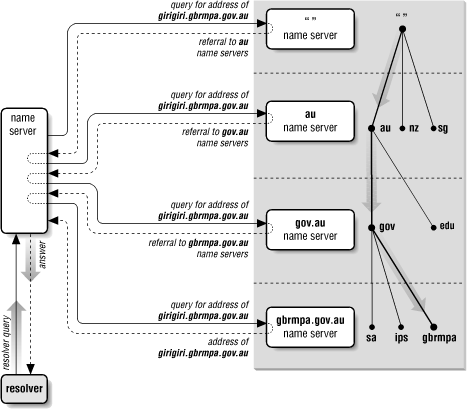
\includegraphics[scale=0.60]{./img/dns-resolution.png}
		\caption{Processo di risoluzione DNS per l'indirizzo di un host di rete. Il client (\emph{resolver}) effettua una query al server DNS locale (o \emph{name server} locale), che si preoccupa poi, in assenza di \emph{cache}, di contattare prima la radice e poi la sequenza di \emph{name server} referenziati necessari per recuperare l'indirizzo richiesto dal client.}
		\label{fig:dns-resolution}
	\end{figure}
\end{description}

\subsection{Struttura gerarchica e modello ad attori} 
\subsubsection{Struttura gerarchica}\label{dns-hierarchy}
Proprio come il \emph{Domain Name System} per gli indirizzi IP, descritto in \autoref{original-dns}, il DNS del sistema Proxima sarà organizzato in maniera gerarchica, con una struttura ad albero rovesciato. In questo caso, però, la risoluzione degli indirizzi non avverrà a partire dai nomi, ma dall'identificativo dei servizi. Ogni servizio è descritto a partire da una sequenza di domini sempre più specifici separati da un punto. Il nome di dominio di un certo nodo viene composto come la sequenza di etichette nel percorso dalla radice dell'albero fino al nodo stesso e non viceversa, come invece illustrato in \autoref{original-dns} (ad esempio \emph{proxima.medical.firstAid}). 

Ogni componente del sistema \emph{Proxima} è caratterizzato dal servizio che mette a disposizione e dall'indirizzo tramite il quale può essere contattato. La separazione in domini del servizio permette la costruzione di un modello strutturato, nel quale solamente gli elementi situati nel settore inferiore dell'albero siano a conoscenza dell'informazione vera e propria, ovvero l'indirizzo del servizio. I nodi superiori della gerarchia possono, invece, rappresentare i domini che descrivono il servizio, consentendo di ottenere un quadro complessivo simile a quello raffigurato in \autoref{fig:dns-hierarchy}.

\begin{figure}[H]
	\centering
	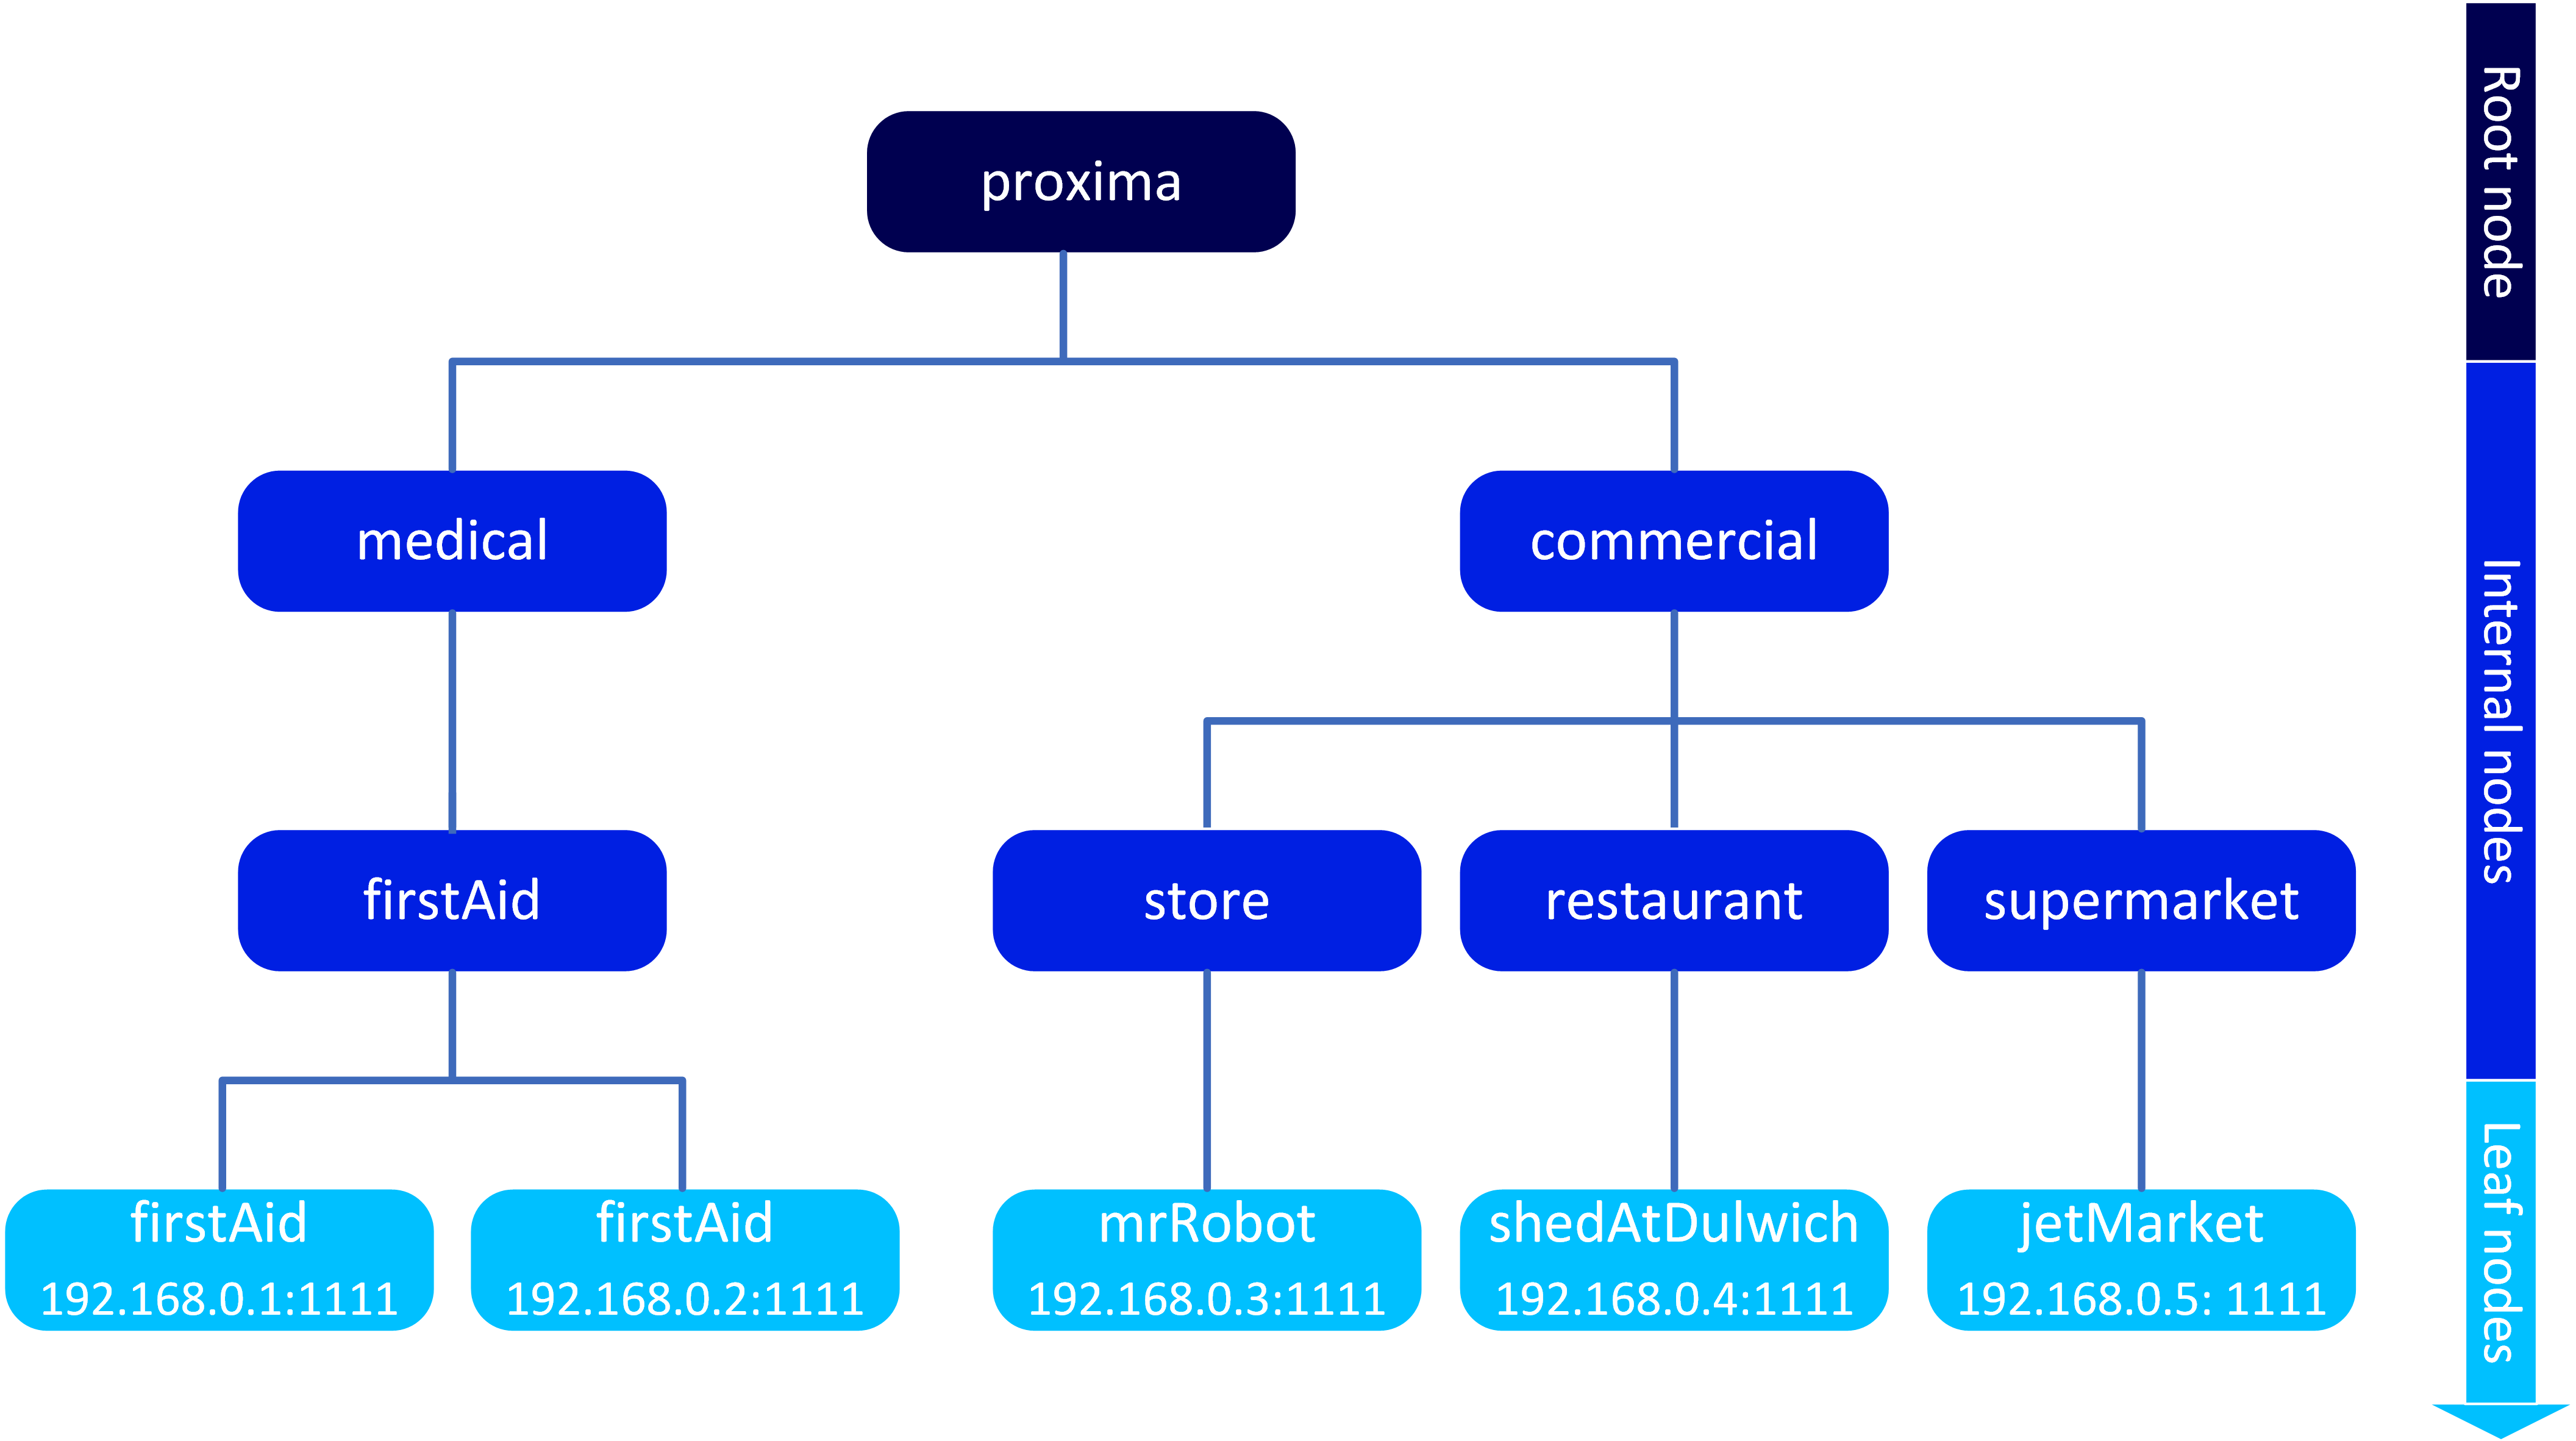
\includegraphics[scale=0.7]{./img/dns-hierarchy.png}
	\caption{Un esempio di struttura gerarchica, ad albero rovesciato, del sistema. Il sotto-albero derivante dal nodo interno \emph{firstAid} è quello di interesse diretto per il progetto in esame. Il sotto-albero derivante dal nodo interno \emph{commercial} non rappresenta un dominio attualmente gestito dal sistema \emph{Proxima}, ma è stato inserito per rappresentare una gamma di servizi che potrebbero potenzialmente essere aggiunti, in maniera dinamica, al DNS, entrando a far parte del sistema. }
	\label{fig:dns-hierarchy}
\end{figure}

Come si può evincere dallo schema in \autoref{fig:dns-hierarchy}, la gerarchia ad albero rovesciato è composta da tre differenti tipologie di nodi:
\begin{itemize}
	\item \textbf{Root node}: è la radice dell'albero, nonché il nodo da cui dovranno transitare tutte le richieste inerenti al DNS. Ad essa è associato il dominio più generale del sistema in esame, ovvero \emph{proxima}, dato che tale dominio dovrà essere condiviso da tutti i servizi del mondo \emph{Proxima}. Può avere un numero arbitrario di figli che, in linea teorica, potrebbero essere sia nodi interni che foglie dell'albero. Per mantenere una visione il più possibile strutturata dei servizi, sarebbe opportuno evitare un legame diretto fra questo nodo e le foglie, delegando la gestione degli indirizzi dei servizi a nodi più specifici.
	\item \textbf{Internal node}: è un nodo interno dell'albero, discendente da un nodo padre (che potrebbe essere un nodo radice o un nodo interno). È caratterizzato dal legame con almeno un nodo figlio (che potrebbe essere sia un nodo foglia, sia un ulteriore nodo interno). Questo nodo può essere considerato come un punto di \emph{routing}, in quanto è in grado di dirottare una certa richiesta di indirizzo verso il nodo più appropriato, che potrebbe essere una foglia che è in grado di soddisfare direttamente la richiesta, oppure un nodo interno tramite il quale sarà poi possibile giungere alla foglia desiderata. Ogni nodo interno è relativo ad un particolare dominio più o meno specifico e si occupa della gestione di tutti i componenti che offrono i servizi appartenenti al dominio di competenza.
	\item \textbf{Leaf node}: è un nodo foglia dell'albero, discendente da un nodo padre (presumibilmente un nodo interno, ma anche un nodo radice in alcuni casi). È uno dei nodi terminali dell'albero, in quanto non può avere figli ed è il custode del contenuto informativo del servizio di competenza. Infatti, ogni nodo foglia è caratterizzato da una corrispondenza diretta verso uno ed un solo componente del sistema \emph{Proxima}, rappresentato per mezzo del servizio che offre, oltre all'indirizzo utilizzabile per stabilire una comunicazione con esso.
\end{itemize}

Questo architettura gerarchica prevede una suddivisione delle informazioni relative ai servizi fra nodi diversi, che potrebbero anche risiedere su componenti fisici separati. Non è prevista la presenza di un nodo universale che condensi al suo interno tutte le informazioni dell'intero sistema \emph{Proxima}, ma si mira alla definizione di un insieme di nodi complementari, che singolarmente hanno una conoscenza limitata della totalità dei servizi, ma presi nel loro insieme garantiscono tutte le funzionalità del servizio DNS desiderato, fornendo anche ampie garanzie di scalabilità.

Nel contesto dei microservizi, adottato come riferimento per il progetto in esame, ogni nodo della struttura gerarchica potrebbe, in una visione estrema, essere considerato come un microservizio, contattabile dai nodi situati in un livello superiore della gerarchia in caso di necessità.

\subsubsection{Modello ad attori} \label{dns-actormodel}
Durante la fase di definizione della struttura gerarchica del servizio DNS, si è posta l'enfasi sulla suddivisione del carico di lavoro tra una moltitudine di nodi attivi e indipendenti. Ognuno di essi è caratterizzato dall'\emph{encapsulation} di uno stato interno e dalla capacità di contattare gli altri nodi della gerarchia, in modo da costruire un sistema collettivo che sia grado di far fronte alle richieste esterne, garantendo scalabilità al crescere del numero dei componenti del sistema \emph{Proxima}. L'analisi di queste prerogative porta ad individuare nel modello ad attori la scelta più appropriata per l'implementazione del servizio.

Si prevede la costruzione di un sistema ad attori nel quale ogni nodo della gerarchia sarà mappato in un corrispondente attore. Se ne deriva la definizione degli attori \emph{DNSRootActor}, \emph{DNSInternalNodeActor} e \emph{DNSLeafNodeActor} che corrispondono rispettivamente a nodo radice, nodo interno e nodo foglia della gerarchia DNS, ognuno relativo ad un dominio del sistema Proxima. I primi due attori condividono la funzionalità di \emph{routing}, necessaria per conservare un riferimento agli attori figli, in modo da poterli contattare in caso di necessità. Ad ogni \emph{DNSLeafNodeActor} sarà invece assegnato l'indirizzo di un determinato componente, oltre al servizio da esso offerto. La comunicazione fra gli attori della gerarchia segue la modalità \emph{message passing}, tratto distintivo del modello ad attori.

L'attore \emph{DNSRootActor} dovrà essere attivo e raggiungibile in ogni momento successivo al deployment del servizio, mentre i nodi interni e le foglie della gerarchia potranno essere creati dinamicamente solo in caso di necessità, seguendo un approccio \emph{by-need}. Questo vincolo pone il problema di costruzione della gerarchia DNS in maniera incrementale durante tutta la fase di esecuzione del sistema. Si prevede, dunque, la presenza di un attore \emph{DNSNodesCreatorActor}, il cui unico scopo consisterà nella creazione di attori \emph{DNSInternalNodeActor} e \emph{DNSLeafNodeActor}, quando adeguatamente sollecitato. Ognuno di questi attori potrà essere creato in un qualsiasi momento durante l'esecuzione del sistema e dovrà inserirsi immediatamente all'interno della gerarchia DNS preesistente. 

\subsection{Interfaccia di comunicazione} \label{dns-communication}
L'interazione con il servizio DNS, come precedentemente stabilito, dovrà essere \emph{RESTful}. Ciò impone la presenza di un server HTTP, il cui scopo sarà quello di soddisfare le richieste esterne giunte in corrispondenza di una determinata porta. Più nel dettaglio, ogni richiesta al DNS dovrà essere diretta alla porta 1406, con l'indicazione del path \emph{dns/address}, che mostra come ogni possibile operazione agisca su un determinato indirizzo di un servizio del sistema \emph{Proxima}. Infatti il punto chiave di un'architettura REST consiste nel modello delle risorse che, nel caso specifico, sono proprio gli indirizzi dei vari servizi del sistema. Ogni richiesta verso il DNS sarà relativa ad una determinata risorsa, che potrà essere richiesta, creata o eliminata. I metodi del protocollo HTTP gestiti dal server DNS sono i seguenti:
\begin{itemize}
	\item \textbf{GET}: messaggio che richiede lo stato di una certa risorsa, individuata tramite l'indicazione di un servizio nell'\emph{URL} della richiesta. Il server DNS risponderà con un messaggio contenente l'indirizzo di un componente che offre il servizio specificato. \newline Si prevede che questa operazione sarà la più utilizzata, in quanto permetterà ad un componente esterno di contattare un servizio del sistema \emph{Proxima} in modo disaccoppiato. Gli unici prerequisiti risultano essere la conoscenza del tipo di servizio offerto dal servizio \emph{Proxima} e la raggiungibilità del DNS.
	\item \textbf{POST}: messaggio che presuppone la richiesta di creazione di una risorsa, descritta nel body della richiesta. Nel caso specifico, la risorsa in questione è l'indirizzo di un componente del sistema \emph{Proxima}. Il server DNS procederà alla creazione dell'indirizzo, rispondendo al client con un apposito \emph{URL}, utilizzabile per richiedere la nuova risorsa. \newline Questa operazione permette l'aggiunta dinamica di servizi al sistema \emph{Proxima}, anche in una fase successiva al deployment. Infatti, sarà possibile inserire un nuovo servizio nel DNS in qualsiasi momento ed esso entrerà immediatamente a far parte del sistema, diventando raggiungibile da un qualsiasi componente richiedente tale servizio al DNS. Inoltre, per garantire un maggiore livello di autonomia, questa operazione potrebbe essere effettuata direttamente da ogni servizio \emph{Proxima}, in una fase immediatamente successiva alla creazione. In questo modo ogni servizio che volesse entrare a far parte del sistema, dovrebbe semplicemente preoccuparsi di registrarsi al DNS indicando il servizio offerto e l'indirizzo utilizzabile per stabilire una comunicazione.
	\item \textbf{DELETE}: messaggio che sollecita l'eliminazione di una risorsa, specificata nella richiesta. Il server DNS provvederà alla rimozione della risorsa, che non sarà più considerata per le future richieste di tipo GET. \newline Questa operazione può risultare utile per informare il DNS che un certo componente non è più disponibile ad offrire il servizio dichiarato, oppure che l'indirizzo precedentemente assegnatogli non è più valido.
\end{itemize}
Una maggiormente approfondita descrizione delle \emph{REST APIs} del server DNS è stata effettuata mediante l'ausilio del framework \emph{Swagger}\footnote{\url{https://swagger.io/}}. Essa è resa disponibile online al link \url{https://app.swaggerhub.com/apis/gmp/ProximaDNSService/1.0.0}.

Lo scopo del server sarà quello di restare in ascolto sulla porta predefinita, demandando alla gerarchia DNS il compito di soddisfare tutte le richieste ricevute. Si rivela opportuna la definizione di un attore \emph{BridgeActor}, in grado di frapporsi fra server e gerarchia interna. In particolare, il compito di questo attore è quello di mappare una richiesta giunta dal server in un corrispondente messaggio comprensibile alla gerarchia interna ed effettuare successivamente il processo inverso, convertendo la risposta elaborata dalla gerarchia interna in un messaggio accessibile al server.

\subsection{Comportamento}
In \autoref{dns-communication} sono state individuate tutte le modalità di interazione con il servizio DNS, sotto forma di metodi HTTP. Dall'analisi di tali operazioni si possono discernere le tre funzionalità principali che il servizio DNS dovrà essere in grado di fornire, ovvero le operazioni di creazione e cancellazione di uno specifico indirizzo, oltre alla restituzione di un indirizzo corrispondente ad un determinato servizio.

\subsubsection{Richiesta dell'indirizzo di un servizio}
\begin{figure}[H]
	\centering
	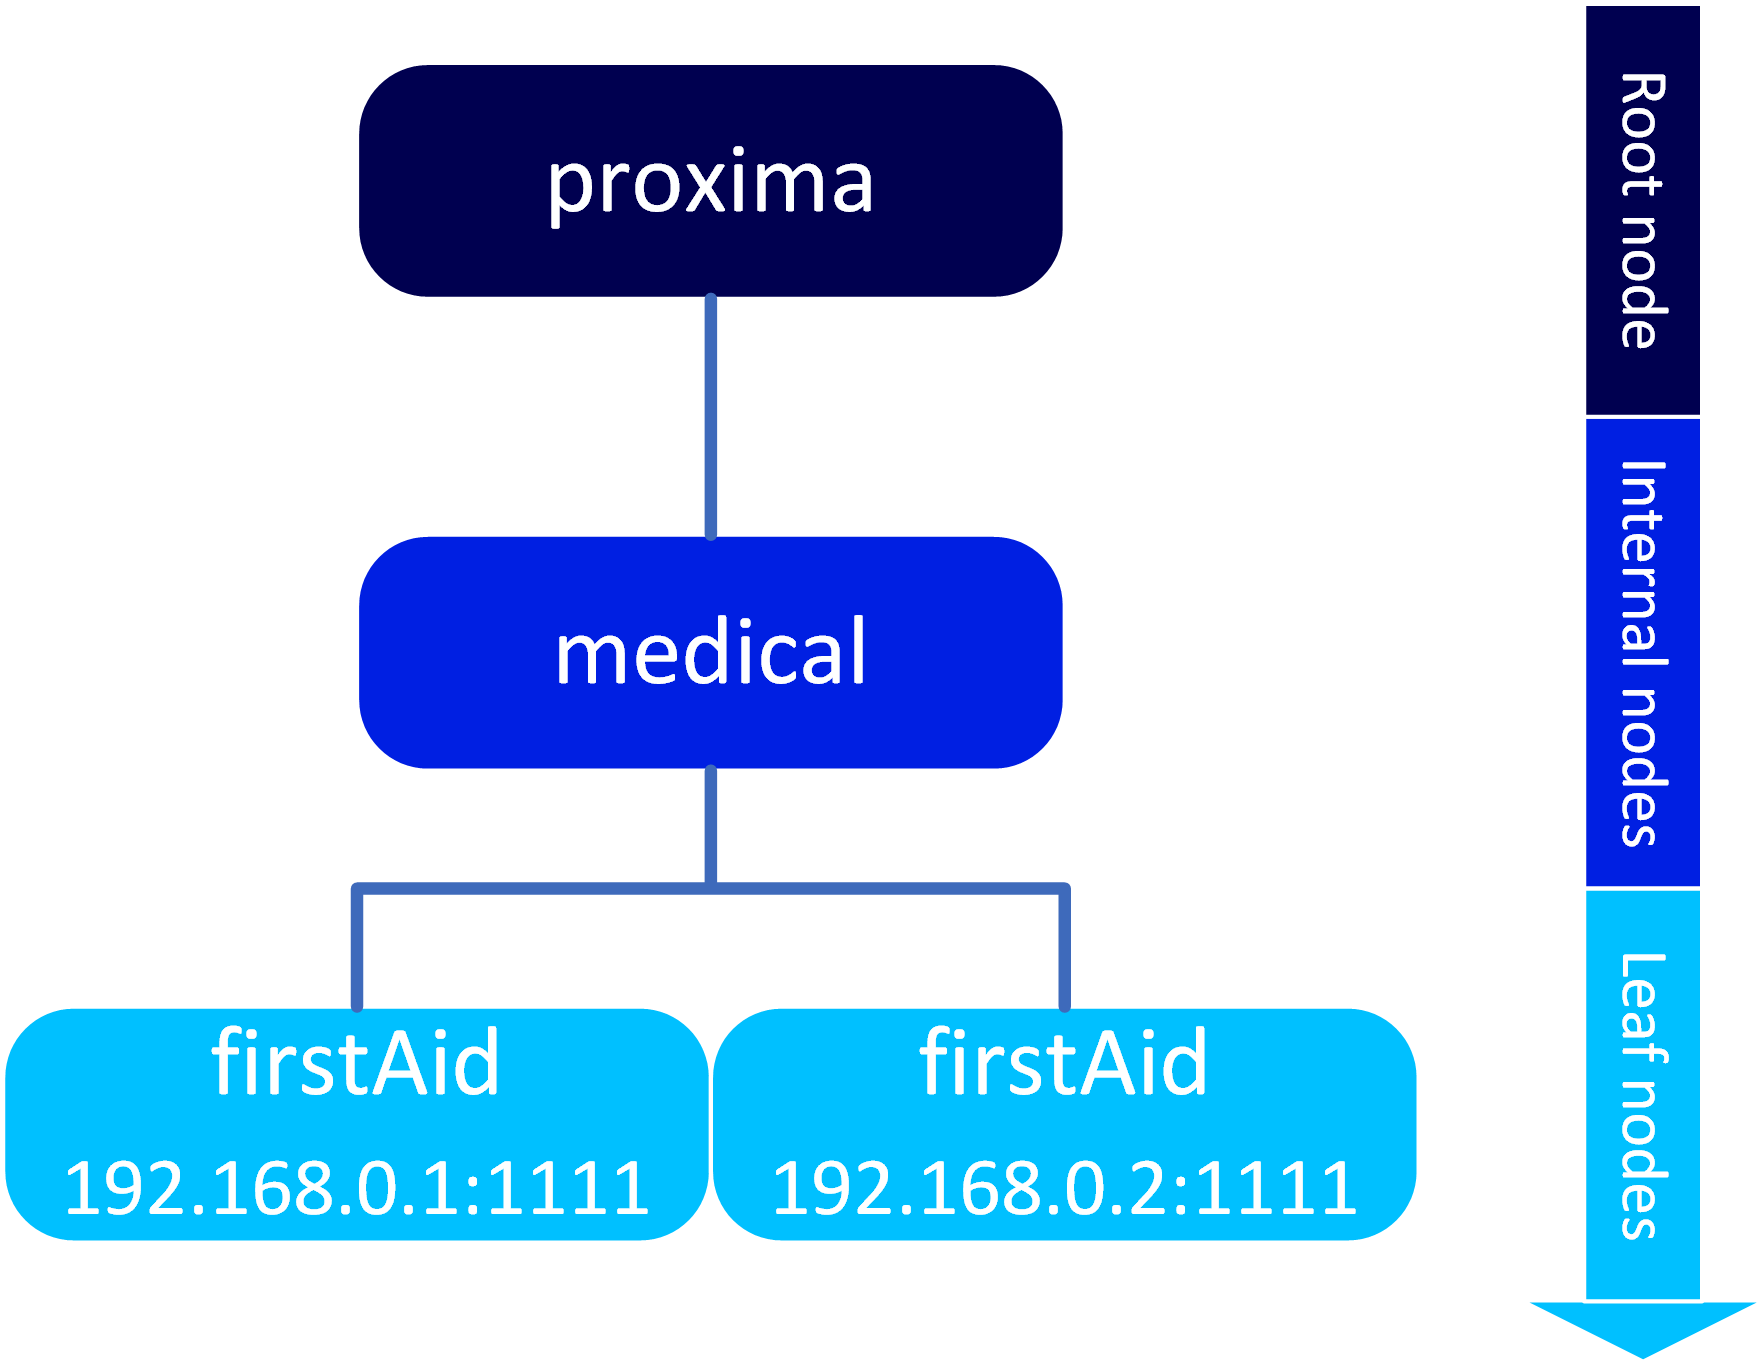
\includegraphics[scale=0.7]{./img/dns-get.png}
	\caption{Un esempio di sviluppo della struttura gerarchica del DNS. Per semplicità si è scelto di considerare solamente l'ambito di interesse specifico del progetto, ovvero il primo soccorso, tralasciando altri possibili domini applicativi del sistema \emph{Proxima}.}
	\label{fig:dns-get}
\end{figure}
In un determinato momento del ciclo di esecuzione del sistema \emph{Proxima}, il DNS sarà provvisto degli indirizzi di un insieme di servizi. Ad esempio, per quanto riguarda l'ambito del primo soccorso, la situazione potrebbe essere simile a quella raffigurata in \autoref{fig:dns-get}. Per garantire scalabilità e disponibilità del sistema generale è ragionevole pensare che un medesimo servizio possa essere offerto da più componenti separati, caratterizzati da un proprio indirizzo individuale. Ognuno di questi componenti dovrà necessariamente essere registrato al DNS, in modo da essere rintracciabile all'interno del sistema \emph{Proxima}. 

Una richiesta dell'indirizzo di un componente in grado di offrire un determinato servizio si riduce ad una ricerca sull'albero DNS di una foglia che sia associata al servizio desiderato. Nel caso si verifichi la presenza di più foglie compatibili con la richiesta (come nel caso in \autoref{fig:dns-get} per il primo soccorso), dovrà essere il DNS stesso a garantire un meccanismo di \emph{load balancing}, in modo da distribuire il carico delle richieste in maniera equa fra i componenti disponibili. Una soluzione semplice ma efficacie consiste nell'implementazione di una politica di \emph{scheduling round-robin}, in cui i componenti possono essere alternati in maniera regolare, evitando il sovraccarico dei singoli nodi.

\subsubsection{Aggiunta dell'indirizzo di un servizio}
\begin{figure}[H]
	\centering
	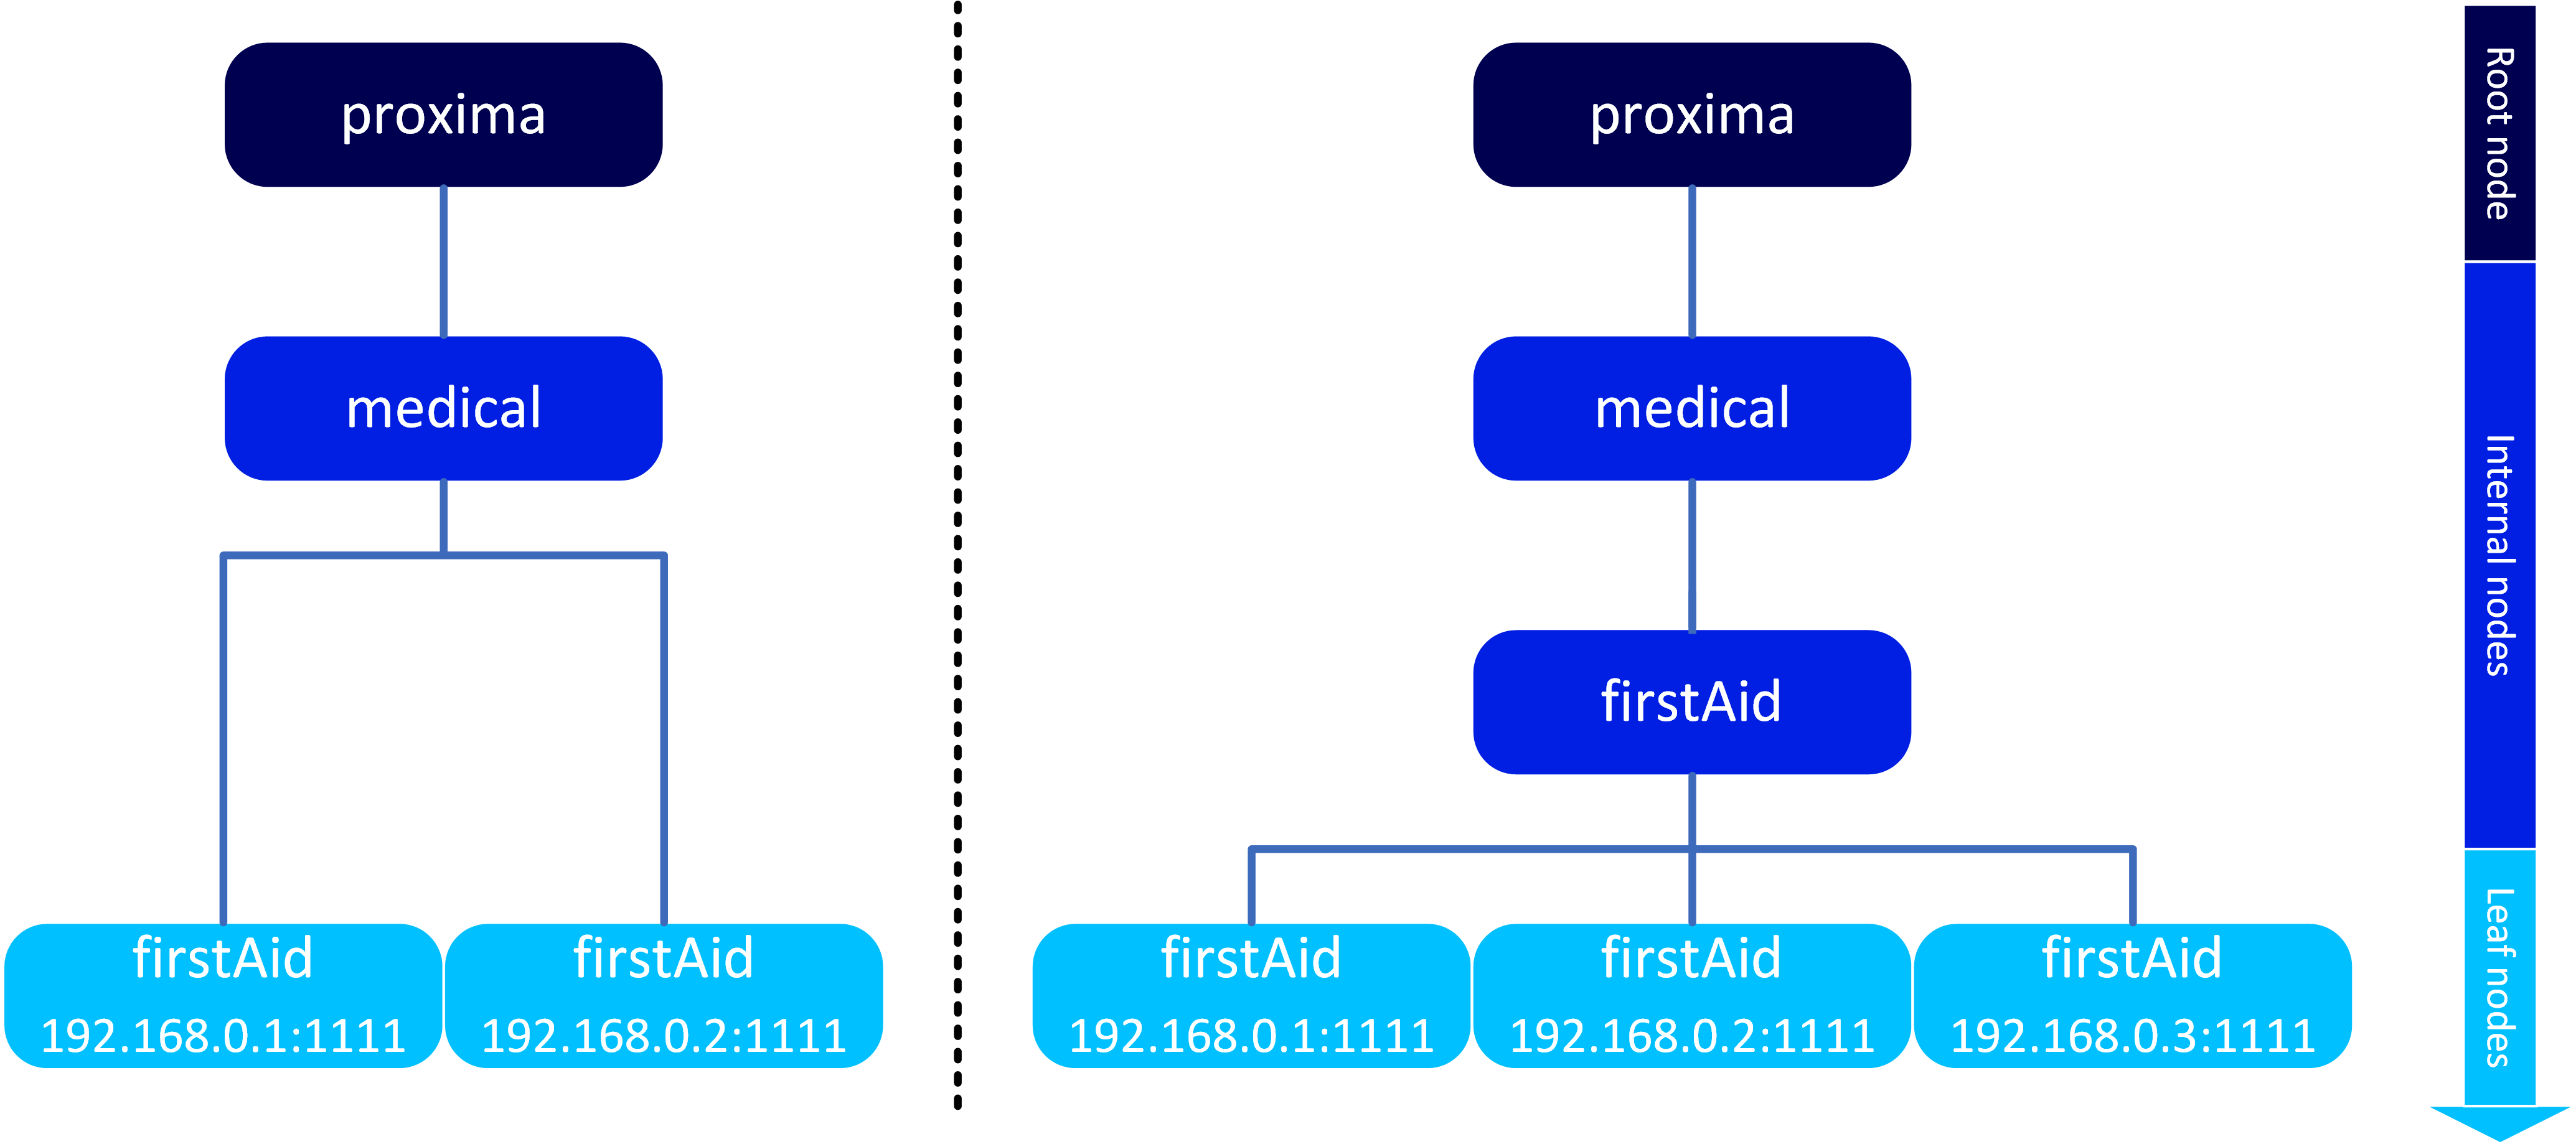
\includegraphics[scale=0.7]{./img/dns-post.png}
	\caption{Nella parte sinistra è raffigurato un esempio di sviluppo della struttura gerarchica del DNS relativa al primo soccorso. Nella parte destra è mostrata l'evoluzione della struttura nel caso in cui un nuovo indirizzo relativo al campo di primo soccorso venisse aggiunto al sistema. }
	\label{fig:dns-post}
\end{figure}
La struttura gerarchica descritta in \autoref{dns-hierarchy} rende molto semplice l'aggiunta dell'indirizzo di un componente che offre un certo servizio. Infatti sarà sufficiente l'aggiunta di una foglia rappresentante il nuovo indirizzo all'albero DNS esistente. 

In \autoref{fig:dns-post} è raffigurato un esempio della struttura DNS prima e dopo l'aggiunta di un nuovo componente appartenente al dominio del primo soccorso al sistema. Si può notare l'introduzione di un nodo interno (\emph{firstAid}), oltre che della nuova foglia. Questo comportamento deriva dal fatto che al raggiungimento di un certo valore di soglia prefissato è opportuno che la gestione di nodi simili (stesso servizio) sia delegata ad un nuovo nodo interno. Nel caso raffigurato, il valore della soglia è posto a 3.

\subsubsection{Eliminazione dell'indirizzo di un servizio}
\begin{figure}[H]
	\centering
	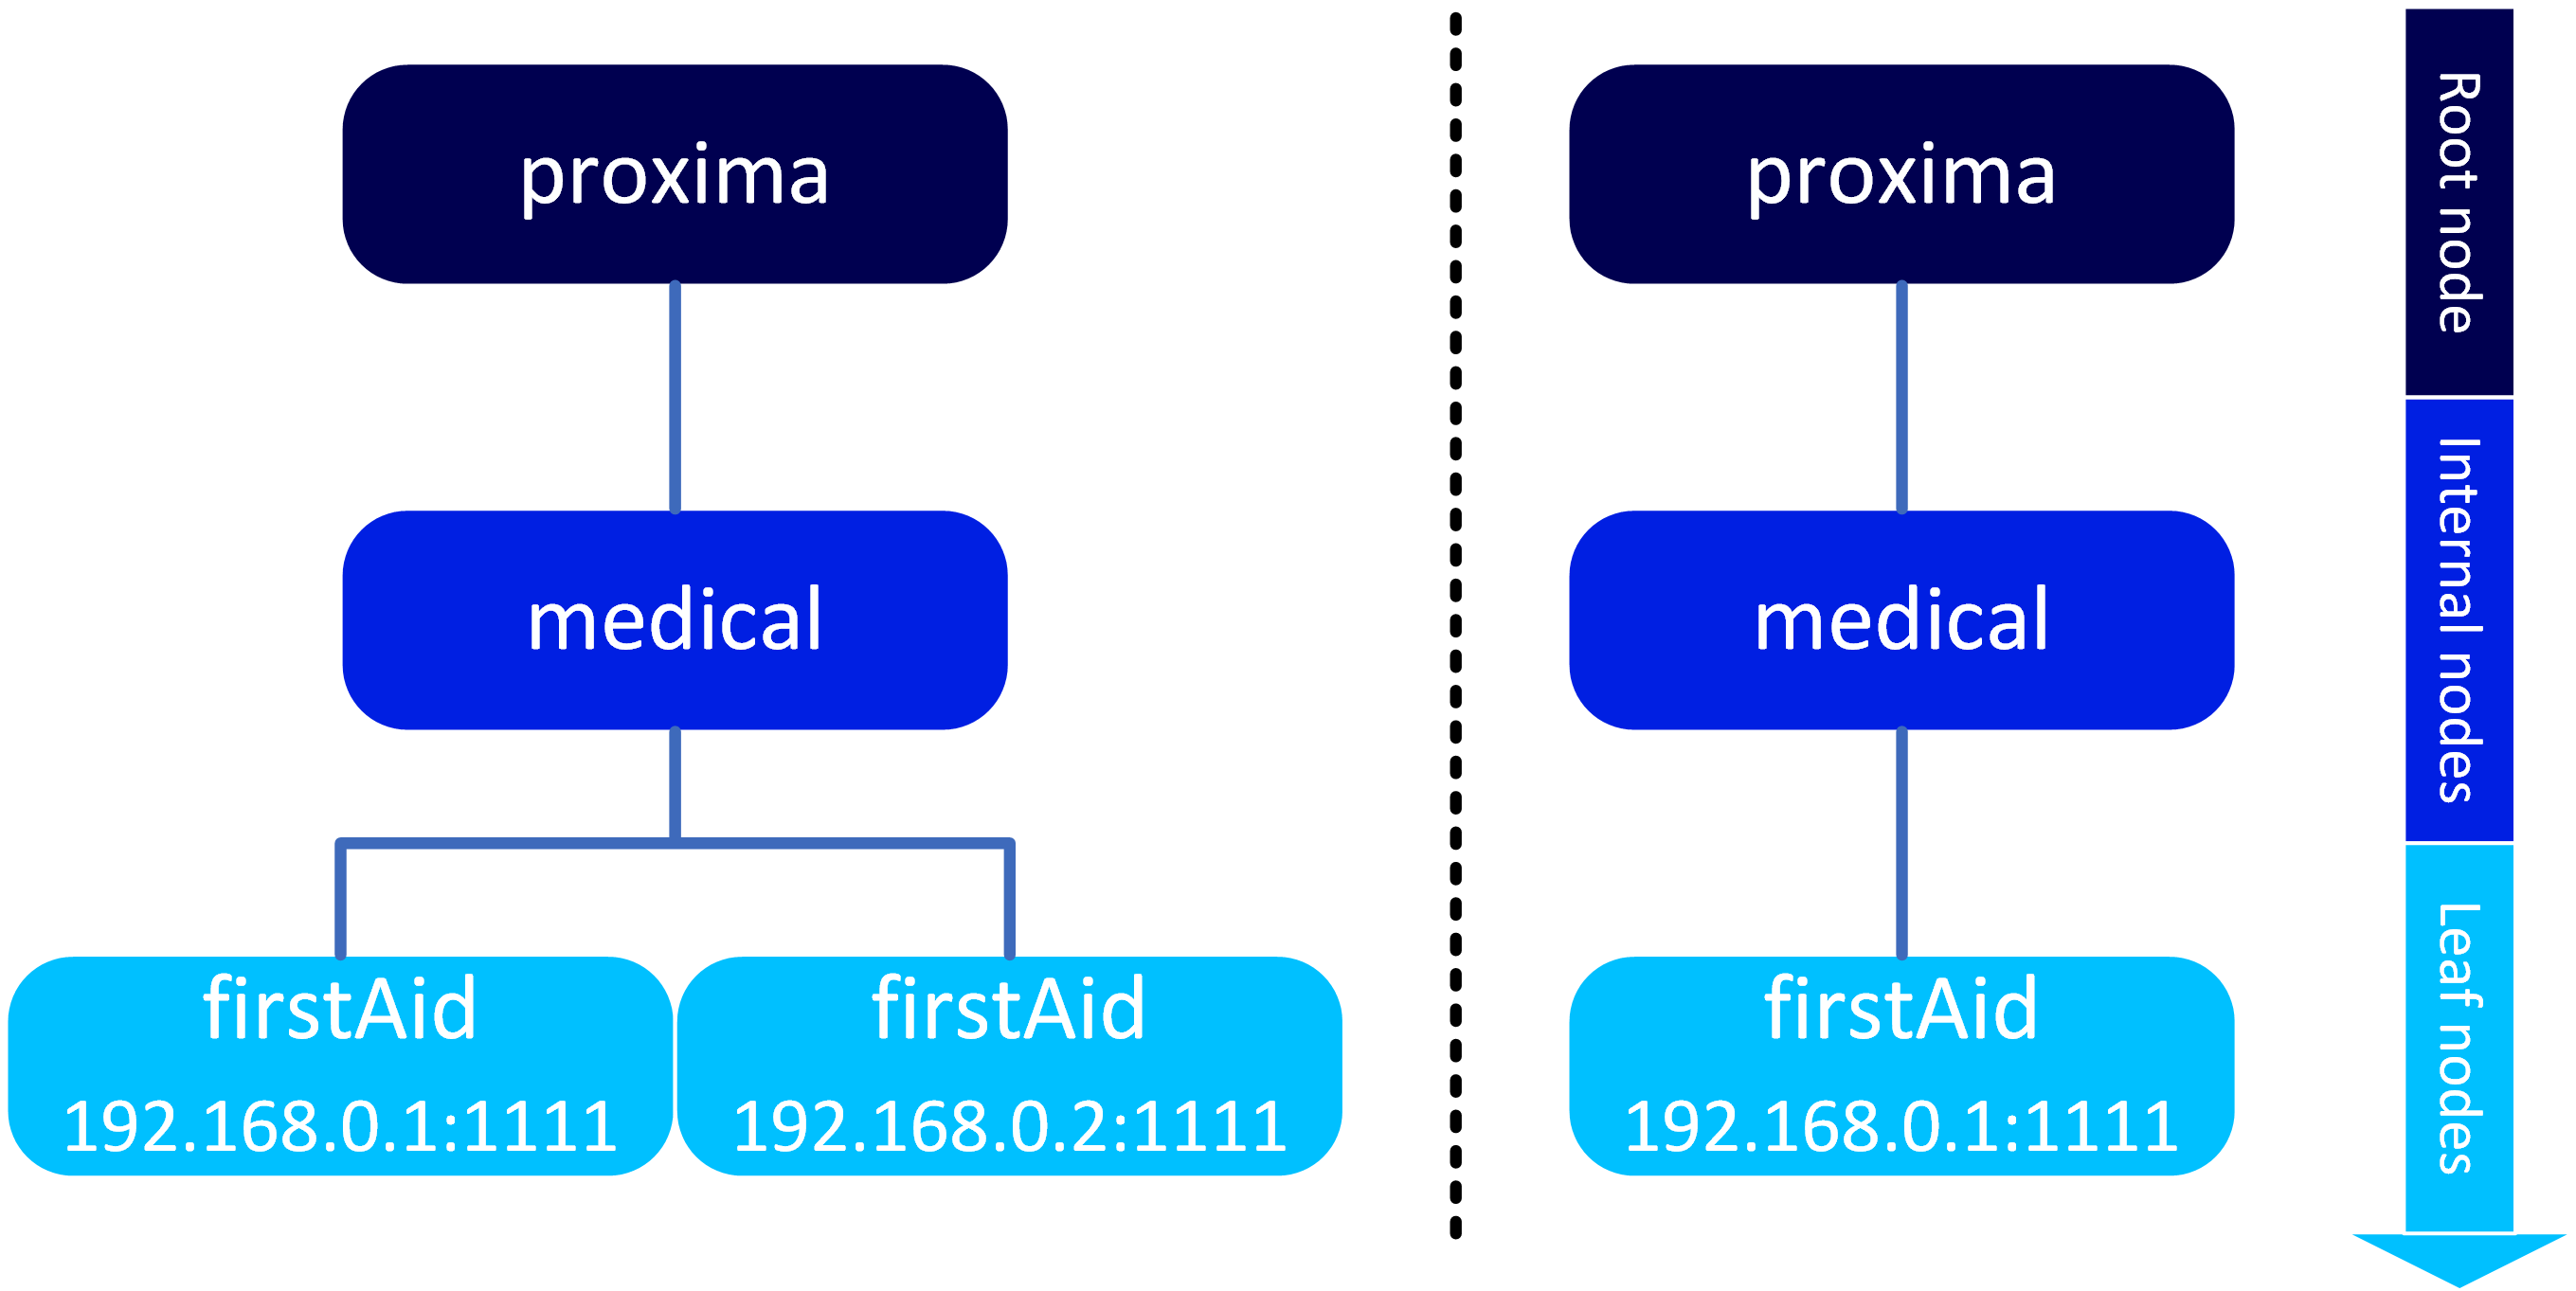
\includegraphics[scale=0.7]{./img/dns-delete.png}
	\caption{Nella parte sinistra è raffigurato un esempio di sviluppo della struttura gerarchica del DNS relativa al primo soccorso. Nella parte destra è mostrata l'evoluzione della struttura nel caso in cui un indirizzo esistente venga eliminato dal sistema (il nodo foglia \emph{firstAid} con indirizzo \emph{192.168.0.2:1111}). }
	\label{fig:dns-delete}
\end{figure}
Se all'interno dell struttura DNS, ogni componente è rappresentato come una foglia dell'albero, la cancellazione di un'indirizzo si riduce all'eliminazione della foglia ad esso corrispondente. 

In \autoref{fig:dns-delete} è mostrato un esempio della struttura DNS prima e dopo l'eliminazione di un componente appartenente al dominio del primo soccorso dal sistema. Si può notare che, nel caso specifico, il servizio di primo soccorso rimarrà comunque garantito all'interno del sistema \emph{Proxima}, in quanto persiste il riferimento ad un altro componente che offre il medesimo servizio. Nel caso così non fosse il servizio non sarebbe più erogabile.

\chapter{Implementazione}

\section{Servizio di autorizzazioni degli utenti}

Il server HTTP, ovvero il servizio in questione, descritto in \autoref{users_authorizations_design} è stato sviluppato in \emph{Node}\footnote{\url{https://nodejs.org/it/}}, facendo affidamento al framework \emph{Espress}\footnote{\url{http://expressjs.com/it/}} ed al linguaggio \emph{Typescript}\footnote{\url{https://www.typescriptlang.org/}}. Oltre al fatto che le tecnologie citate risultano essere fortemente consolidate e supportate, questa scelta è stata fatta principalmente per due motivazioni, quali facilità di sviluppo e largo supporto per l'interazione con database non relazionali.

Per il database finalizzato al contenimento delle autorizzazioni di ogni singolo utente è stato fatto affidamento a \emph{MongoDB}\footnote{\url{https://www.mongodb.com/it}}, essendo questa una delle tecnologie di punta per la creazione e gestione di database non relazionali. Più nel dettaglio, il database contiene una sola collezione, \emph{usersauthorizations}, nella quale ogni documento memorizza l'elenco dei servizi i quali un determinato utente ha autorizzato per l'utilizzo dei propri dati.   

\section{Servizio DNS}
L'implementazione del servizio DNS è completamente basata sulle direttive espresse nella fase di progettazione in \autoref{design-dns}. 

Per lo sviluppo del sistema ad attori, si è fatto uso del
framework \emph{Akka}\footnote{\url{https://akka.io/}}, e degli strumenti da esso forniti. Questa scelta è motivata sia dalle elevate performance (circa 50 milioni di messaggi processati al secondo, oltre alla possibilità di creare fino a 2.5 milioni di attori per GB di heap), sia dalle garanzie offerte dal framework in merito allo sviluppo di sistemi distribuiti e scalabili. In particolare si è fatto uso della libreria \emph{akka-actor} per la costruzione del sistema ad attori della gerarchia DNS, con l'ausilio di \emph{akka-http} (oltre ad \emph{akka-stream}) per implementare con semplicità ed efficacia il server HTTP del servizio. Per quanto riguarda il linguaggio di programmazione, si è scelto di utilizzare \emph{Scala}\footnote{\url{https://www.scala-lang.org/}}, in quanto è il linguaggio adottato per la maggiore nel processo di sviluppo del framework \emph{Akka}, e permette di sfruttarne tutto il 
potenziale.

Seguendo le scelte progettuali, descritte in \autoref{dns-actormodel}, si è deciso di procedere con la definizione dei trait \emph{DNSNodeActor} e \emph{DNSRouterActor}, attraverso la composizione dei quali è stato poi possibile definire le classi di attori \emph{DNSRootActor}, \emph{DNSInternalNodeActor} e \emph{DNSLeafNodeActor}. Il trait \emph{DNSNodeActor} rappresenta un nodo della gerarchia (nodo interno o foglia) e si contrappone alla radice, definita, invece, in maniera indipendente. Questa tipologia di attore, nel momento immediatamente successivo alla creazione, prevede l'inserimento nella gerarchia DNS preesistente, tramite l'invio di un messaggio di registrazione alla radice. Il trait \emph{DNSRouterActor} rappresenta un nodo in grado di svolgere una funzione di routing all'interno della gerarchia. Questa tipologia di attore è in grado di gestire la registrazione di un nuovo nodo all'interno della gerarchia, oltre ad instradare le richieste di indirizzi verso le foglie adibite.

Sfruttando la definizione dei trait appena illustrati, le classi di attori corrispondenti ai nodi della gerarchia DNS sono state così composte:
\begin{itemize}
	\item \textbf{DNSRootActor}: specializzazione del trait \emph{DNSRouterActor}.
	\item \textbf{DNSInternalNodeActor}: mixin dei trait \emph{DNSNodeActor} e \emph{DNSRouterActor}, in modo da ottenere un duplice comportamento all'interno della gerarchia.
	\item \textbf{DNSLeafNodeActor}: specializzazione del trait \emph{DNSNodeActor}, dotato della logica di gestione di un indirizzo di un particolare componente del sistema Proxima.
\end{itemize}

L'implementazione del resto del sistema si è rivelata fluida e in linea rispetto a quanto proposto nella fase di progettazione. L'unica eccezione riguarda la creazione automatica dei nodi interni della gerarchia. Per garantire ciò si è rivelata necessaria la definizione di un attore \emph{DNSControllerActor}, che, periodicamente, possa controllare lo stato della gerarchia e, se necessario, ordinare la creazione di uno o più nodi interni al \emph{DNSNodesCreatorActor}.

\section{Applicazione Android}

In questa sezione verranno brevemente discusse le più rilevanti scelte implementative relative all'applicazione Android. In modo da soddisfare tutti i requisiti seguendo al contempo le \emph{guidelines} illustrate in \autoref{design_app}, l'applicazione è stata strutturata in 4 componenti principali:
\begin{enumerate}
	\item \textbf{MainActivity}: una delle due activity dell'applicazione, responsabile della gestione dell'interazione con l'utente. Più nel dettaglio, il suo scopo è quello di abilitare l'avvio e l'interruzione della ricerca di identificatori vicini al dispositivo e guidare il soccorritore nella procedura necessaria al recupero dei dati medici dalla banca dati (\autoref{design_app} - schermate 1, 2, 3). Inoltre, questa activity funge da \emph{listener} per i broadcast generati dal sistema Android alla rilevazione di un tag NFC. La lettura dei tag stessi è delegata ad un componente apposito, descritto in seguito.
	\item \textbf{DataPrinterActivity}: activity avente il solo compito di visualizzare i dati medici una volta recuperati dalla banca dati (\autoref{design_app} - schermata 4). La visualizzazione dei dati medici stessi è stata strutturata cercando di sfruttare per intero il display del dispositivo, in modo che il soccorritore possa consultare ciò di cui più necessita nel minor tempo possibile. 
	\item \textbf{NdefReaderTask}: AsyncTask dedito alla lettura del contenuto dei tag NFC rilevati dal dispositivo. Come accennato in precedenza, la lettura viene eseguita facendo riferimento al formato NDEF (\emph{NFC default exchange format}). Essendo tale operazione delegata a questo componente, l'activity in foreground risulta essere reattiva anche durante la lettura stessa.
	\item \textbf{HTTPClientService}: servizio \emph{bounded} alla \emph{MainActivity}, responsabile dell'interazione con il front server. Il suo compito è quindi quello di inviare richieste ben formattate al server e di notificare la \emph{MainActivity} a fronte della ricezione di risposte. Il servizio in esame fa affidamento alla libreria \emph{Volley} per l'invio di richieste e la ricezione di risposte su HTTPS.
\end{enumerate}

Sia chiave pubblica del front server che chiave privata del soccorritore sono contenute all'interno della cartella \emph{assets} del progetto, e caricate a runtime di conseguenza. In una versione non prototipale dell'applicazione, sarebbe d'obbligo migliorare la gestione, perlomeno, della chiave privata, facendo in modo che non sia facilmente accessibile tramite \emph{tool} di de-compilazione. 

Infine, siccome in ambiente Android non è nativamente possibile considerare le letture di tag NFC solo dopo, come nel nostro caso, la pressione di un pulsante, la \emph{MainActivity} è stata strutturata in modo da rendere possibile questo filtraggio.  

\chapter{Testing} 
\section{Servizio DNS}
L'implementazione del servizio DNS è stata accompagnata dalla costante definizione di test, finalizzati soprattutto alla verifica della correttezza dei singoli attori definiti. È stato adottato l'approccio di \emph{unit testing}, attraverso il quale ogni attore soggetto a test è stato isolato dal resto del sistema e testato singolarmente tramite dei meccanismi offerti dalla libreria \emph{akka-testkit}. Essa ha permesso di interrogare gli attori a tempo di esecuzione e definire delle asserzioni sulla base dei messaggi con essi scambiati, attraverso dei costrutti di libreria come \emph{expectMsg}, oltre ai classici \emph{assert}. 

Oltre agli attori del sistema, anche il server DNS è stato opportunamente testato mediante l'ausilio della libreria \emph{akka-http-testkit}, che ha permesso, in modo molto semplice e immediato, la simulazione di richieste HTTP, in modo da poter valutare la correttezza del comportamento del server in reazione ai messaggi esterni.

In generale, ogni test è stato architettato grazie all'utilizzo della libreria \emph{scalatest}, che, tramite la composizione di trait diversi (ad esempio \emph{WordSpecLike} e \emph{Matchers}) ha dato la possibilità di utilizzare frasi di senso compiuto, unite a parole chiave (es: \emph{must} oppure \emph{in}), per costruire dei test facilmente
leggibili e comprensibili, sia in fase di realizzazione che di esecuzione.

\section{Applicazione Android}

Per la quasi totalità delle componenti software dell'applicazione Android sono state sviluppate delle apposite classi di testing in modo da convalidarne il funzionamento. Più nello specifico, per le classi \emph{android-independent} è stato fatto affidamento al framework \emph{JUnit}\footnote{\url{https://junit.org/junit4/}} per la scrittura dei relativi test, situati all'interno della cartella \texttt{test}. Per quanto riguarda invece le classi \emph{android-related} (come \emph{Activitis, Services, \dots}) è stato fatto ricorso alla scrittura di \emph{instrumented tests} attraverso la libreria \emph{Espresso}\footnote{\url{https://developer.android.com/training/testing/espresso/index.html}}, che ha comodamente permesso di verificare il corretto funzionamento delle interfacce utente così come il funzionamento delle componenti in background. Questa seconda categoria di test è situata all'interno della cartella \texttt{androidTest}. Purtroppo non è stato creato un test automatizzato per la classe \emph{org.gammf.proxima.NdefReaderTask} per via dell'impossibilità di simulare la lettura di un tag NFC.

\chapter{Deployment}

In questo capitolo verrà trattato il \emph{deployment} del sistema nella sua interezza, considerando le varie alternative presenti per i vari componenti che lo compongono.

\section{Microservizi}

La suddivisione del sistema in microservizi apre diverse possibilità per il \emph{deployment} del sistema stesso:
\begin{itemize}
	\item \textbf{Distribuzione dei microservizi}: ogni microservizio può potenzialmente essere installato su di una macchina diversa, in modo da garantire il massimo disaccoppiamento tra i microservizi stessi. La gestione degli indirizzi delle macchine non sarebbe un problema, in quanto facilmente gestiti dal servizio DNS.
	\item \textbf{Replicazione dei microservizi}: qualora necessario, si potrebbe decidere di replicare uno o più servizi, procedendo ad installarli sulla stessa macchina o su una macchina differente. Alla creazione, una replica, per entrare a far parte del sistema, dovrebbe semplicemente registrarsi (tramite una richiesta POST) al servizio DNS. Questo approccio porterebbe ad una migliore gestione delle richieste volte ai servizi di interesse, bilanciando il carico delle stesse. Inoltre, la presenza di repliche migliorerebbe notevolmente le caratteristiche di \emph{fault-tollerance} e \emph{availabilty} del sistema. Infatti, un malfunzionamento di un componente non inciderebbe sul funzionamento del sistema nel caso fosse presente almeno un altro componente che offrisse il medesimo servizio. Anche qui, l'utilizzo di questo approccio non creerebbe problemi per la gestione degli indirizzi, per via della presenza del servizio DNS.
\end{itemize}

In un'ottica più generale, l'aggiunta di nuovi servizi al sistema risulta essere facile ed immediata: come accennato in precedenza, il servizio appena creato dovrebbe solo registrarsi al servizio di DNS.

Per garantire un maggior livello di sicurezza all'interno del sistema, è opportuno che solamente il \emph{front server} sia contattabile dall'esterno. I microservizi saranno quindi mantenuti all'interno dei confini di una rete privata non accessibile da Internet. In questo modo, un utente che desidera fruire del servizio sarà vincolato a contattare il \emph{front server}, il quale potrà invece interrogare i microservizi necessari per esaudire la richiesta dell'utente.

Come ultima nota, la distribuzione del servizio DNS avverrà tramite un file JAR (\emph{Java ARchive}).
 
\section{Front server}

L'interfacciamento al sistema \emph{Proxima} può avvenire solamente per mezzo del componente \emph{front server}, al quale saranno indirizzate tutte le richieste provenienti dagli utenti. Esso può essere quindi visto come collo di bottiglia del sistema e avrà il duplice scopo di rimanere reattivo anche a fronte di un carico elevato di richieste e, allo stesso tempo, contattare i vari microservizi interni al sistema per elaborare le risposte corrispondenti. In condizioni reali d'utilizzo del sistema, è ragionevole presupporre che il carico di lavoro sul componente in questione sarà elevato, dato che il sistema sarà utilizzato a livello nazionale ed eventualmente esteso con ulteriori servizi. Sulla base di questa considerazione, si valuta come ideale una soluzione che prevede un deployment del componente su cloud. Questo approccio garantisce un servizio continuo ed elastico, con un'allocazione di risorse dinamica sulla base del carico di richieste. Inoltre, essa consente un risparmio economico notevole, in quanto non sarebbe necessario procedere all'acquisto di un server dedicato in grado di garantire prestazioni elevate.

\section{Applicazione Android}

L'applicazione Android verrà distribuita tramite un file in formato \emph{apk}. Idealmente essa dovrebbe essere fruibile ai soli soccorritori autorizzati. Quindi, la soluzione più intuitiva consiste nell'installazione manuale nell'\emph{apk} nei singoli dispositivi del personale autorizzato. Siccome da requisito è prevista anche la fornitura dei dispositivi, essi potrebbero essere distribuiti con l'applicazione preinstallata. Questo approccio presenta però il seguente problema: non essendo l'applicazione su sistemi di distribuzione di uso comune (come \emph{Google Play Store}\footnote{\url{https://play.google.com/store/apps?hl=it}}) viene reso non praticabile l'aggiornamento automatico dell'applicazione stessa.
Ovviamente, un aggiornamento manuale dell'applicazione su tutti i dispositivi è da escludere. Per questo motivo si è deciso inizialmente di effettuare il deployment dell'applicazione su \emph{Google Play Store}. Nonostante l'applicazione, in questo modo, sia potenzialmente utilizzabile da chiunque, qualunque soggetto non autorizzato non sarebbe in grado di svolgere alcuna operazione di rilievo con essa. Per rendere l'applicazione effettivamente fruibile ai soli soccorritori autorizzati, si potrebbe creare un microservizio in grado di fornire la versione più aggiornata dell'applicazione ai quei dispositivi che la richiedono, a patto che su questi sia installata una versione precedente dell'applicazione stessa.

L'unico problema di rilievo riguarda la chiave privata del soccorritore, che, al primo avvio dell'applicazione, dovrà essere inserita manualmente da un ente autorizzato. 

\chapter{Manutenzione}

In questo capitolo verrà eseguito uno studio sulla manutenibilità del sistema. Più nello specifico, saranno analizzati alcuni dei possibili cambiamenti che sarebbe ragionevole apportare al sistema in futuro, assieme a nuove eventuali direttive del committente che porterebbero alla modifica di determinati componenti del sistema stesso. Per ognuna di queste ne verrà indicato l'impatto e la relativa facilità di effettuazione.

\section{Richieste del committente}

Riuscire a prevedere tutte le possibili richieste che il committente potrebbe avanzare in futuro risulta essere un compito molto difficile. In questa sezione ci si limita quindi ad eseguire un'analisi di quelle principali, riportate di seguito:
\begin{itemize}
	\item \textbf{Cambiamento delle tecnologie}: è presumibile pensare che in futuro il committente possa richiedere di sostituire l'identificatore degli utenti con uno più evoluto. Questo potrebbe accadere se, ad esempio, venisse creata una tecnologia in grado di far comunicare lettore e identificatore in un raggio limitato di 3 metri (come da requisito iniziale). Il cambio di identificatore comporterebbe un cambio del protocollo di comunicazione tra i componenti citati. Per affrontare questo cambiamento, si potrebbe modificare l'applicazione Android, in termini di dipendenze e librerie utilizzate, in modo da affiancare al supporto per NFC quello per la nuova tecnologia, a patto che ciò sia possibile. In caso contrario, risulterebbe necessario sostituire l'applicazione Android con un lettore \emph{ad-hoc}, rendendo il cambiamento più costoso e complesso. Come alternativa, nel caso fosse possibile si potrebbero invece utilizzare degli identificatori \emph{ad-hoc} in grado di essere letti sia tramite NFC, sia tramite la nuova tecnologia; in questo modo si potrebbe perlomeno continuare ad utilizzare l'applicazione Android. Qualunque sia l'approccio scelto, ci si limiterebbe ad agire su lettori ed identificatori, senza apportare alcuna modifica alle componenti restanti del sistema, come \emph{front server} e microservizi.  
	
	\item \textbf{Metodo di autenticazione}: per garantire un maggior livello di sicurezza in relazione alla consultazione dei dati da parte di personale autorizzato, il committente potrebbe richiedere di apportare modifiche al metodo di autenticazione del personale stesso. Per esempio, al posto di utilizzare identificativo del soccorritore si potrebbe voler utilizzare una sua caratteristica biometrica (volto, voce, \dots). Innanzitutto, tale richiesta prevederebbe una modifica all'applicazione Android, in modo che sia possibile, con essa, effettuare il riconoscimento della caratteristica biometrica di interesse. In seguito, per minimizzare l'impatto del cambiamento sul sistema, basterebbe creare un servizio dedito al mapping da caratteristica biometrica ad identificativo. A questo punto, l'applicazione Android si limiterebbe ad interagire con il sistema al solito modo, inviando, in ogni richiesta, un pattern che descriva la caratteristica biometrica utilizzata al posto dell'identificativo utilizzato in precedenza. Il \emph{front server}, a seguito della ricezione di una richiesta così formattata, provvederà a contattare il nuovo servizio in modo da ottenere l'identificativo di interesse, per poi procedere al recupero dei dati medici. 

	Sulla base di quanto appena detto, non sarebbe quindi necessaria alcuna modifica alla struttura o ai servizi del sistema. Tuttavia, il cambiamento avrebbe impatto decisamente maggiore qualora il riconoscimento della caratteristica biometrica scelta dal committente non fosse supportato da Android. In tal caso, occorrerebbe sostituire l'applicazione con un lettore \emph{ad-hoc}, assicurandosi che questo sia in grado di leggere il contenuto degli identificatori degli utenti.
	
	\item \textbf{Interfaccia al sistema}: in futuro il committente potrebbe richiedere di sviluppare un'app iOS analoga a quella Android, o, più in generale, fornire vie alternative di interfacciamento al sistema, come \emph{web app} o sito web. L'unico costo derivante da questa richiesta starebbe nella realizzazione del nuovo componente; per fare in modo di integrare il componente stesso nel sistema, baserà infatti far sì che questo comunichi con il \emph{front server} inviando richieste GET opportunamente formattate. L'aggiunta di una nuova interfaccia al sistema non andrebbe quindi ad intaccare struttura del sistema stesso e/o microservizi.
\end{itemize}

\section{Evoluzione del sistema}

Il punto di forza del sistema sta nella sua architettura a microservizi. Sebbene per poterla attuare sia stato fatto del lavoro aggiuntivo in fase di progettazione, questa architettura comporta una serie di vantaggi in termini di scalabilità, estensibilità e manutenibilità del sistema. Di seguito sono riportati ed analizzati alcuni cambiamenti facilmente applicabili in un'ottica di evoluzione del sistema:
\begin{itemize}
	\item \textbf{Replicazione/eliminazione microservizi}: qualora in futuro un determinato servizio del sistema \emph{Proxima} presentasse un aumento notevole del proprio utilizzo, si potrebbe semplicemente decidere di replicare i microservizi finalizzati all'erogazione del servizio di interesse. L'integrazione delle repliche all'interno del sistema sarebbe, come già accennato precedentemente in questo documento, a costo zero; basterebbe infatti che le repliche, a tempo di creazione, si registrassero al servizio DNS (con un'apposita richiesta POST) per poter poi essere contattate da chi ne necessita.
	
	Contrariamente, nel caso un determinato servizio del sistema presentasse un forte calo nel suo utilizzo, si potrebbe considerare di eliminare eventuali repliche dei microservizi finalizzati all'erogazione del servizio di interesse. Anche quest'operazione risulterebbe immediata, siccome sarebbe sufficiente che le repliche da eliminare venissero de-registrate dal servizio di DNS (con un'apposita richiesta DELETE).
	
	\item \textbf{Tecnologia dei microservizi}: qualora in futuro risultasse vantaggioso apportare modifiche ad un certo microservizio o, più in generale, utilizzare un'altra tecnologia per la sua implementazione, allora queste operazioni evolutive sarebbero limitate al solo microservizio di interesse, senza andare ad impattare sul sistema e sull'interazione tra i suoi componenti. Sarà sufficiente infatti che l'interfaccia del microservizio in esame rimanga la stessa, in modo che gli altri componenti del sistema possano continuare ad interagire con esso come in precedenza. Questo discorso relativo ai microservizi risulta valido anche per il \emph{front-server}.
\end{itemize}  

\chapter{Restrospettiva}
\section{Giudizio finale}
\section{Sviluppi futuri}

 
\end{document}
